% Nejprve uvedeme tridu dokumentu s volbami
\documentclass[czech,bachelor]{diploma}
% Dalsi doplnujici baliky maker
\usepackage[autostyle=true,czech=quotes]{csquotes} % korektni sazba uvozovek, podpora pro balik biblatex
\usepackage[backend=biber, style=iso-numeric, alldates=iso]{biblatex} % bibliografie
\let\biblatexaddspace\addspace

\usepackage{dcolumn} % sloupce tabulky s ciselnymi hodnotami
\usepackage{subfig} % makra pro "podobrazky" a "podtabulky"
\usepackage[cpp]{diplomalst}

\usepackage{comment}
\usepackage{imakeidx}
\usepackage[miktex]{gnuplottex}
\usepackage{graphicx}
\usepackage{musixtex}
\usepackage{calligra}
\usepackage{punk}
\usepackage{foekfont}

\makeindex[columns=1, title=Rejstřík, intoc]

% Zadame pozadovane vstupy pro generovani titulnich stran.
\ThesisAuthor{Adam Šárek}

\ThesisSupervisor{Ing. Svatopluk Štolfa, Ph.D.}

\CzechThesisTitle{Virtuální sdílená tabule}

\EnglishThesisTitle{Whiteboard Online Sharing Tool}

\SubmissionYear{2021}

\CzechAbstract{Cílem této práce je vytvoření moderní, responzivní webové aplikace sdílené virtuální tabule. Práce se zaměřuje na optimalizaci pro plynulý chod aplikace a umožňuje tak spolupráci více uživatelů. Důraz je kladen také na podporu více typů zařízení. Práce se inspiruje několika existujícími weby, které dále rozšiřuje. Aplikace nabízí jednoduché nástroje, které umožňují její využití v širokém spektru oblastí. Každá tabule má dva základní režimy přístupu (úpravy a zobrazení), z nichž každý má svůj vlastní odkaz. Výsledkem práce je funkční řešení pro vytváření a sdílení virtuálních tabulí.}

\CzechKeywords{API; Canvas API; Fetch API; WebSockets; MySQL; JSON; Web workers; HTML; JavaScript; PHP}

\EnglishAbstract{The goal of this work is to create a modern, responsive web application for a shared virtual whiteboard. The work focuses on optimization for the smooth running of the application and thus allows the cooperation of multiple users. Emphasis is also placed on supporting multiple types of devices. The work is inspired by several existing sites, which it further extends. The application offers simple tools that allow its use in a wide range of areas. Each whiteboard has two basic access modes (editing and viewing), each with its own link. The result is a functional solution for creating and sharing virtual whiteboards.}

\EnglishKeywords{API; Canvas API; Fetch API; WebSockets; MySQL; JSON; Web workers; HTML; JavaScript; PHP}

\AddAcronym{API}{Application Programming Interface}
\AddAcronym{JSON}{JavaScript Object Notation}
\AddAcronym{HTML}{Hyper Text Markup Language}
\AddAcronym{DOM}{Document Object Model}
\AddAcronym{URL}{Uniform Resource Locator}
\AddAcronym{PHP}{PHP: Hypertext Preprocessor}

\addbibresource{Bibliography.bib}

% Novy druh tabulkoveho sloupce, ve kterem jsou cisla zarovnana podle desetinne carky
\newcolumntype{d}[1]{D{,}{,}{#1}}

% Sloppypar without changing indentation
\newenvironment{sloppypar*}{\sloppy\ignorespaces}{\par}

% Dalsi vrstva zanoreni
\newcommand{\subsubsubsection}[1]{\paragraph{#1}\mbox{}\\\noindent}

% Podpora jazyka JavaScript v lstlisting
\lstdefinelanguage{JavaScript}{
	morekeywords=[1]{ break, continue, delete, else, for, function, if, in, new, return, this, typeof, var, void, while, with },
	% Literals, primitive types, and reference types.
	morekeywords=[2]{ false, null, true, boolean, number, undefined, Array, Boolean, Date, Math, Number, String, Object },
	% Built-ins.
	morekeywords=[3]{ eval, parseInt, parseFloat, escape, unescape },
	sensitive,
	morecomment=[s]{/*}{*/},
	morecomment=[l]//,
	morecomment=[s]{/**}{*/}, % JavaDoc style comments
	morestring=[b]',
	morestring=[b]"
}[keywords, comments, strings]


% Zacatek dokumentu
\begin{document}

% Nechame vysazet titulni strany.
\MakeTitlePages

% A nasleduje text zaverecne prace.
\chapter{Úvod}
\label{chap:1}
Motivací práce bylo vytvořit moderní responzivní webovou aplikaci pro sdílení virtuální tabule, která bude umožňovat spolupráci více uživatelů na různých typech zařízení.
Virtuální tabule slouží k zaznamenávání a sdílení návrhů a ilustrací pomocí jednoduchých nástrojů, díky kterým je možné ji využít v práci, škole či v osobním životě.
%je oblast využití tohoto řešení skutečně široká.
Samotný obsah tabule je průběžně synchronizován, takže jsou změny jednotlivých uživatelů vidět přímo bez nutnosti stránku aktualizovat.
Zároveň jsou také veškeré úpravy ukládány do databáze, která slouží jako trvalé uložiště dat a také záloha při případném výpadku serveru či spojení.
%Databáze je poté využita pro načítání obsahu při připojení uživatele a také jako záloha při případném výpadku serveru či spojení.

%Myšleno je také na případné problémy, které se mohou vyskytnout nejen na straně uživatele, ale také na straně serveru.
%Samotný obsah tabule je průběžně synchronizován a ukládán, takže při výpadku sítě či serveru je po obnovení spojení vždy načten poslední uložený stav.
%, tak aby při , každopádně toto řešení nabízí také export pomocí obrázku či zdrojového souboru, kdykoli možné 
První kapitola se věnuje výběru jednotlivých stávajících řešení nástrojů pro sdílení virtuální tabule.
Kapitola uvádí nástroje a technologie vybraných webů a porovnává je s vypracovaným řešením.

Druhá kapitola se zaměřuje na rozbor požadavků, analýzu problémů a možných řešení a také na architekturu systému.
Kapitola přibližuje vnitřní strukturu systému na kterém je celé řešení postaveno.

Třetí kapitola pak pojednává o implementaci samotného řešení a jeho jednotlivých součástí.
Nejprve je zmíněno vykreslování, jeho optimalizace pomocí vláken a také zpracování barev v rámci barevných motivů.
Dále se kapitola věnuje výměně dat mezi klientských zařízením a serverem pomocí WebSockets.
Následně je popsána správa dat, která na lokální či serverové úrovni zajišťuje využití dat pro konkrétní potřeby uživatele.
Zmíněno je mimo jiné využití MySQL databáze, LocalStorage a Fetch API a také jednotlivé možnosti exportování tabule do rastrové či nativní podoby.
V poslední řadě se kapitola věnuje uživatelskému rozhraní z pohledu responzivity, podpory více jazyků včetně jejich zakomponování do sdílení tabule a také jednotlivým stránkám a jejich podobě ve finálním řešení.
%, ať už lokální či serverová zahrnuje využití MySQL databáze, LocalStorage či Fetch API a je pak dále včetně exportu tabule detailně popsána.
%S daty se lokálně i na serveru dále pracuje a tento proces je pak dále popsán včetně využití MySQL databáze, LocalStorage či Fetch API.  jsou následně ukládána do MySQL databáze či LocalStorage, což je také podrobně popsáno.
%Serverová i lokální správa dat je pak dále popsána včetně využití MySQL databáze a LocalStorage.
%začátek vývoje řešení, kdy 
%pojednává o využití Canvas API, coby plnohodnotné technologie pro vykreslování grafického výstupu na webu.
%Kapitola obsahuje popis této technologie včetně ukázky několika příkladů základních funkcí.

%Třetí kapitola se zaměřuje na výměnu dat mezi klientským zařízením a serverem pomocí protokolu WebSocket.
%Tento protokol poskytuje snadný a spolehlivý přenos dat, což umožňuje interaktivní spolupráci více uživatelů.

%Čtvrtá kapitola se věnuje správě dat a popisuje dva základní způsoby jak lze data ukládat či načítat pro další využití.
%Popsáno je využití MySQL databáze, kde data zůstávají uloženy dlouhodobě mezi jednotlivými návštěvami webu a dále pak exportování a nahrání dat v nativní podobě ve formátu JSON.

%Pátá kapitola rozšiřuje předchozí kapitoly o pohled na optimalizaci jednotlivých příkazů a dat, což umožňuje plynulejší chod webové aplikace.
%Zmiňuje se mimo jiné o Web workers použitých k rozdělení instrukcí do více vláken či o různých změnách v datech pro konkrétní místa použití.

%Poslední kapitola se zaměřuje na nedokončené části bakalářské práce a jejich možné rozšíření či vylepšení.
\endinput
\chapter{Inspirace řešení}
\label{chap:2}
Virtuální sdílená tabule je natolik užitečný nástroj, že je na internetu již spousta různých variant řešení.
Odlišit se tedy není snadné, a proto je práce inspirována několika již existujícími weby, které v rámci funkcí rozšiřuje o určité nové nápady.




\section{Analýza vybraných webů}
\label{sec:2.1}
Weby použité pro inspiraci bylo nejdříve potřeba analyzovat jak z hlediska uživatelských nástrojů a rozhraní, tak z hlediska použitých technologií pro dosažení výsledné funkčnosti.
K identifikaci použitých technologií bylo využito standardně zabudovaných vývojářských nástrojů webového prohlížeče, konkrétně v tomto případě prohlížeče Mozilla Firefox ve verzi 86.
Pro inspiraci bylo vybráno celkově pět webů, které jsou níže vypsány od nejméně po nejvíce autorově subjektivně vnímané ideální řešení nástroje pro sdílení virtuální tabule.




\section{Inspirace vybranými weby}
\subsection{Inspirace - classroomscreen.com}
\label{sec:2.2}
Jako první proběhla analýza webu \underline{classroomscreen.com}.
Tato stránka již na první pohled vypadá spíše jako sdílená obrazovka než jako sdílená tabule, což ostatně napovídá i její název.
Obrazovka zobrazuje simulaci jednotlivých oken, které slouží jako kalendář, stopky, generátor hodu kostkou a další.
Jednotlivé okna mají velmi odlišnou funkčnost a působí tedy podobným dojmem jako počítačové aplikace, což umožňuje tento web využít pro velmi různorodé účely.
Rozhraní obsahuje několik základních tlačítek nástrojů pro vytvoření již zmíněných instancí oken.
Na pozadí je od prvního spuštění vykreslen náhodný obrázek většinou s motivem přírody či nějaké kulturní památky, který je možné kdykoliv změnit v nastavení.
Web má jasně vymezené okraje použitelné části plochy, které jsou dané velikostí uživatelova okna prohlížeče.
Není tedy možné se pohybovat libovolně mimo viditelnou oblast.
Web není určen pro spolupráci více uživatelů a je tedy vhodný především pro menší projekty či prezentace.
Jedinou technologií, která stojí za zmínku je zde Canvas API, která je použita k vykreslování grafického výstupu.
\begin{sloppypar*}
Inspirací k bakalářské práci byl tento web pouze díky nástroje pro úpravu poznámek.
Poznámka v bakalářské práci je stejně jako na tomto webu tvořena pomocí Canvasu překrytého HTML elementem \texttt{<div>} využívajícím atribut \texttt{contenteditable="true"}, který umožňuje úpravu vnitřního textu a díky čemuž tato poznámka působí celistvým dojmem.
\end{sloppypar*}
\begin{figure}[h!]
	\centering
	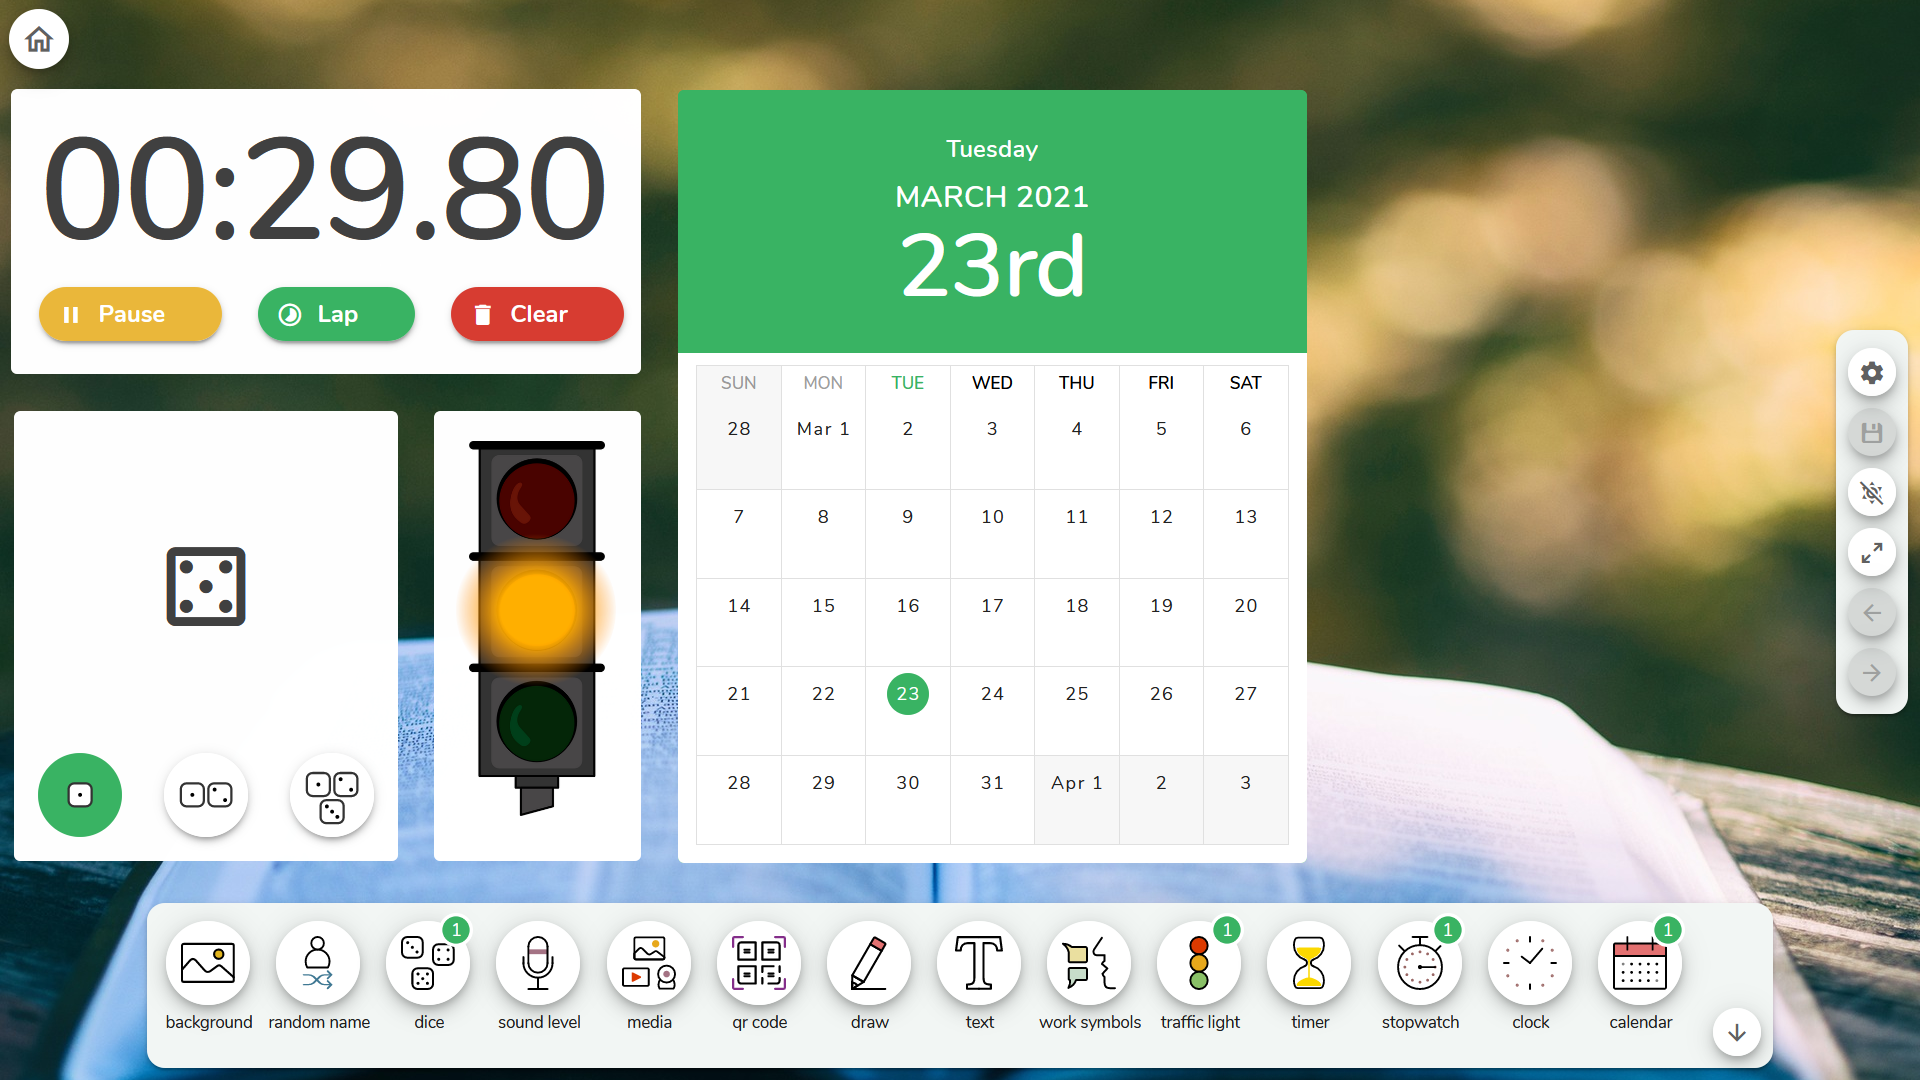
\includegraphics[width=1\textwidth]{Figures/classroomscreen.png}
	\caption{Ukázka webu classroomscreen.com}
	\label{fig:classroomscreen}
\end{figure}



\subsection{Inspirace - whiteboard.fi}
\label{sec:2.3}
Dále byla zanalyzována stránka \underline{whiteboard.fi}.
Tento web registrovaný pod finskou národní doménou je orientovaný především pro využití ve školním prostředí.
Po vytvoření místnosti je zobrazeno plátno o předem dané velikosti, které se ostatním uživatelům během úpravy neaktualizuje.
Pro odeslání aktuálního stavu plátna je potřeba stisknout tlačítko Push.
V rámci místnosti je možné vytvářet více pláten a libovolně mezi nimi přepínat a upravovat je.
Web obsahuje základní nástroje jako kreslení, přidání textu, obrázku či speciální nástroje jako notový zápis a další a jak již bylo zmíněno, jeho využití je tedy především ve škole.
Stránka rovněž využívá Canvas API pro vykreslení grafiky, ale navíc používá protokol WebSocket, díky kterému podporuje spolupráci více uživatelů.

Hlavní inspirací u tohoto webu bylo přepínání hustoty mřížky na pozadí plátna, díky které je možné lépe umístit či vyměřit určité objekty.
\begin{figure}[h!]
	\centering
	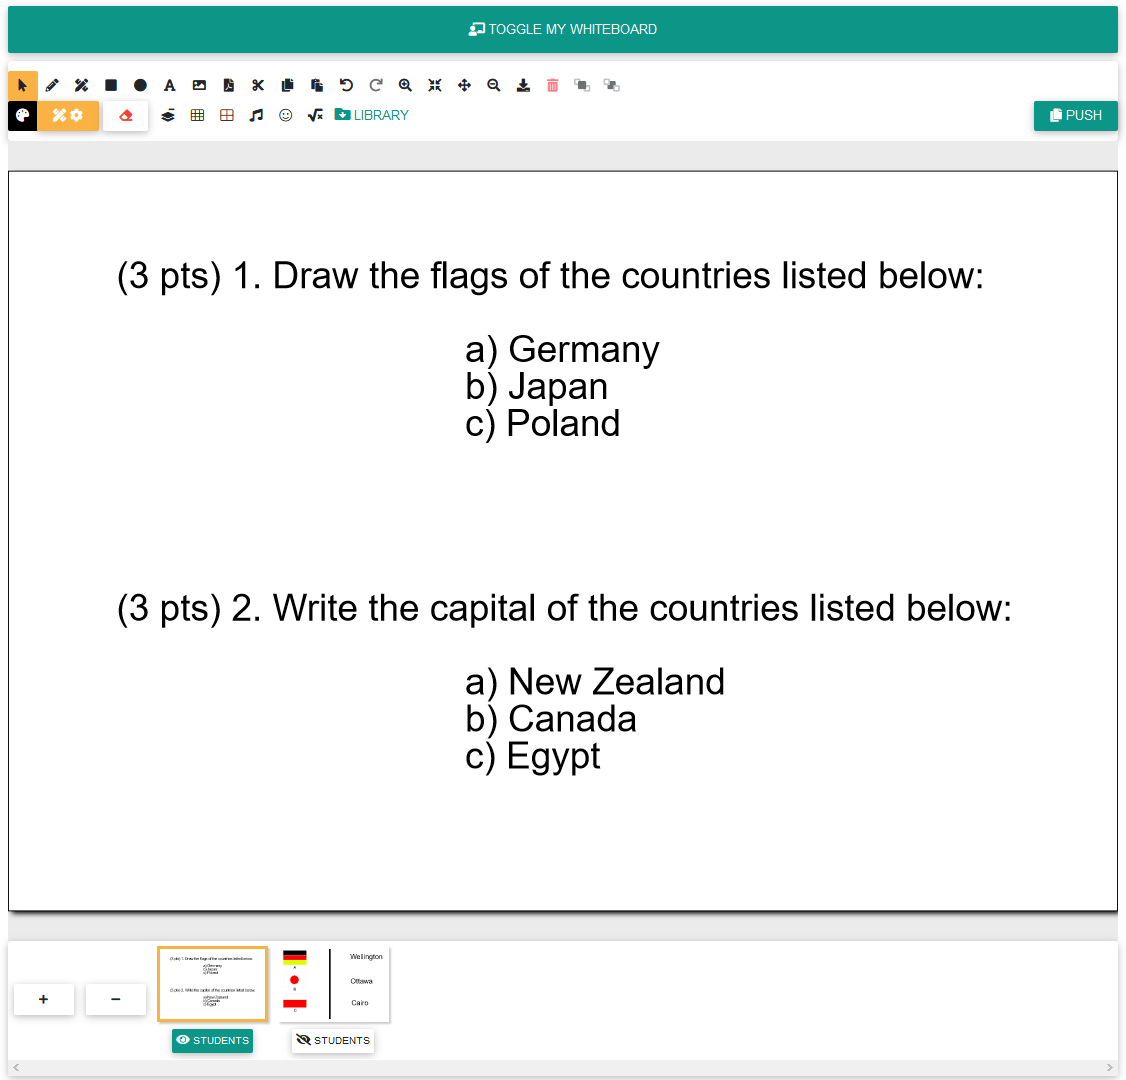
\includegraphics[width=1\textwidth]{Figures/whiteboard.png}
	\caption{Ukázka webu whiteboard.fi}
	\label{fig:whiteboard}
\end{figure}



\subsection{Inspirace - whiteboardfox.com}
\label{sec:2.4}
Třetím webem pro inspiraci byl \underline{whiteboardfox.com}.
Tento web oproti předchozím mnohem více funguje na myšlence virtuální sdílené tabule.

Velikost plátna tabule není omezena velikostí okna prohlížeče a veškeré úpravy tabule jsou automaticky distribuované všem uživatelům.
Inspirace těmito dvěma vlastnostmi jsou ostatně hlavním důvodem, proč je zde tato stránka zmíněna.

Uživatelské rozhraní však nepůsobí příliš moderně, není responzivní a orientace v něm je relativně složitá, jelikož většina nástrojů je schována pod tlačítkem nastavení, což pro mnoho uživatelů nemusí být intuitivní.
Opět se zde objevuje využití Canvasu a také WebSocket, který zmíněný web používá ke sdílení dat a díky čemuž je tento web určen pro spolupráci více uživatelů.



\subsection{Inspirace - collboard.com}
\label{sec:2.5}
Předposledním vybraným řešením virtuální tabule je stránka \underline{collboard.com}.
Tato stránka vylepšuje nedostatky předchozího webu co se týče náročnosti používání uživatelského rozhraní a doplňuje jej o celou řadu možností úprav jednotlivých objektů, jako např. změna tloušťky čáry u kreslení či změna řezu písma u textu a další.
Veškeré objekty lze libovolně vybírat a přesouvat či dále měnit.
Web dále umožňuje přidávat různé pluginy, které využitelnost celého řešení ještě více rozšiřují.
U tabule je možné zadat také její název, což se může zdát jako drobnost, nicméně tento detail může být užitečný pro identifikaci sdílené tabule např. v emailové pozvánce.
Na místě je také tlačítko vrácení na počáteční pozici.
Může se totiž lehce stát, že se uživatel při pohybu po tabuli ztratí.
Použité technologie se oproti předchozímu řešení nijak neliší.

Tento web byl velmi výraznou inspirací pro finální řešení bakalářské práce, jelikož nabízí opravdu moderní, responzivní prostředí, plné užitečných nástrojů a velmi dobře promyšlených řešení případných uživatelských problémů.
Jedná se tak o velmi užitečný nástroj pro sdílení virtuální tabule.



\subsection{Inspirace - miro.com}
\label{sec:2.6}
Nejrozsáhlejší a nejpropracovanější stránkou z výběru je \underline{miro.com}.
Oproti collboard.com je tento web rozšířen o další spoustu nástrojů vhodných pro větší projekty.
Poskytuje vlastní API pro tvorbu pluginů a také integraci s aplikacemi třetích stran jako Microsoft Teams či Google Disk.
Nabízí funkci chatu, seznam poznámek, zobrazuje umístění jednotlivých uživatelů.
Přidávat lze mimo základní nástroje také šablony, tedy např. myšlenkové mapy či vývojové diagramy viz. obrázek \ref{fig:miro} a obsahuje také opravdu detailní konfiguraci jednotlivých objektů.
V rámci technologií kromě Canvasu a WebSocket používá navíc Web worker.
Web worker slouží k rozdělení operací do více vláken, čímž se sníží nároky na hlavní vlákno, které je dle specifikací povinné reagovat na uživatelský vstup. \cite{web:MDN/MainThread}
Touto optimalizací je hlavní vlákno schopno dosáhnout vyššího výkonu, což ve výsledku znamená plynulejší běh celého webu.

Největší inspirací byl vizuální styl uživatelského rozhraní a také způsob sdílení tabule prostřednictvím emailu a rozdělení tabule do různých uživatelských režimů - úpravy a zobrazení.
\begin{sidewaysfigure}[h!]
	\centering
	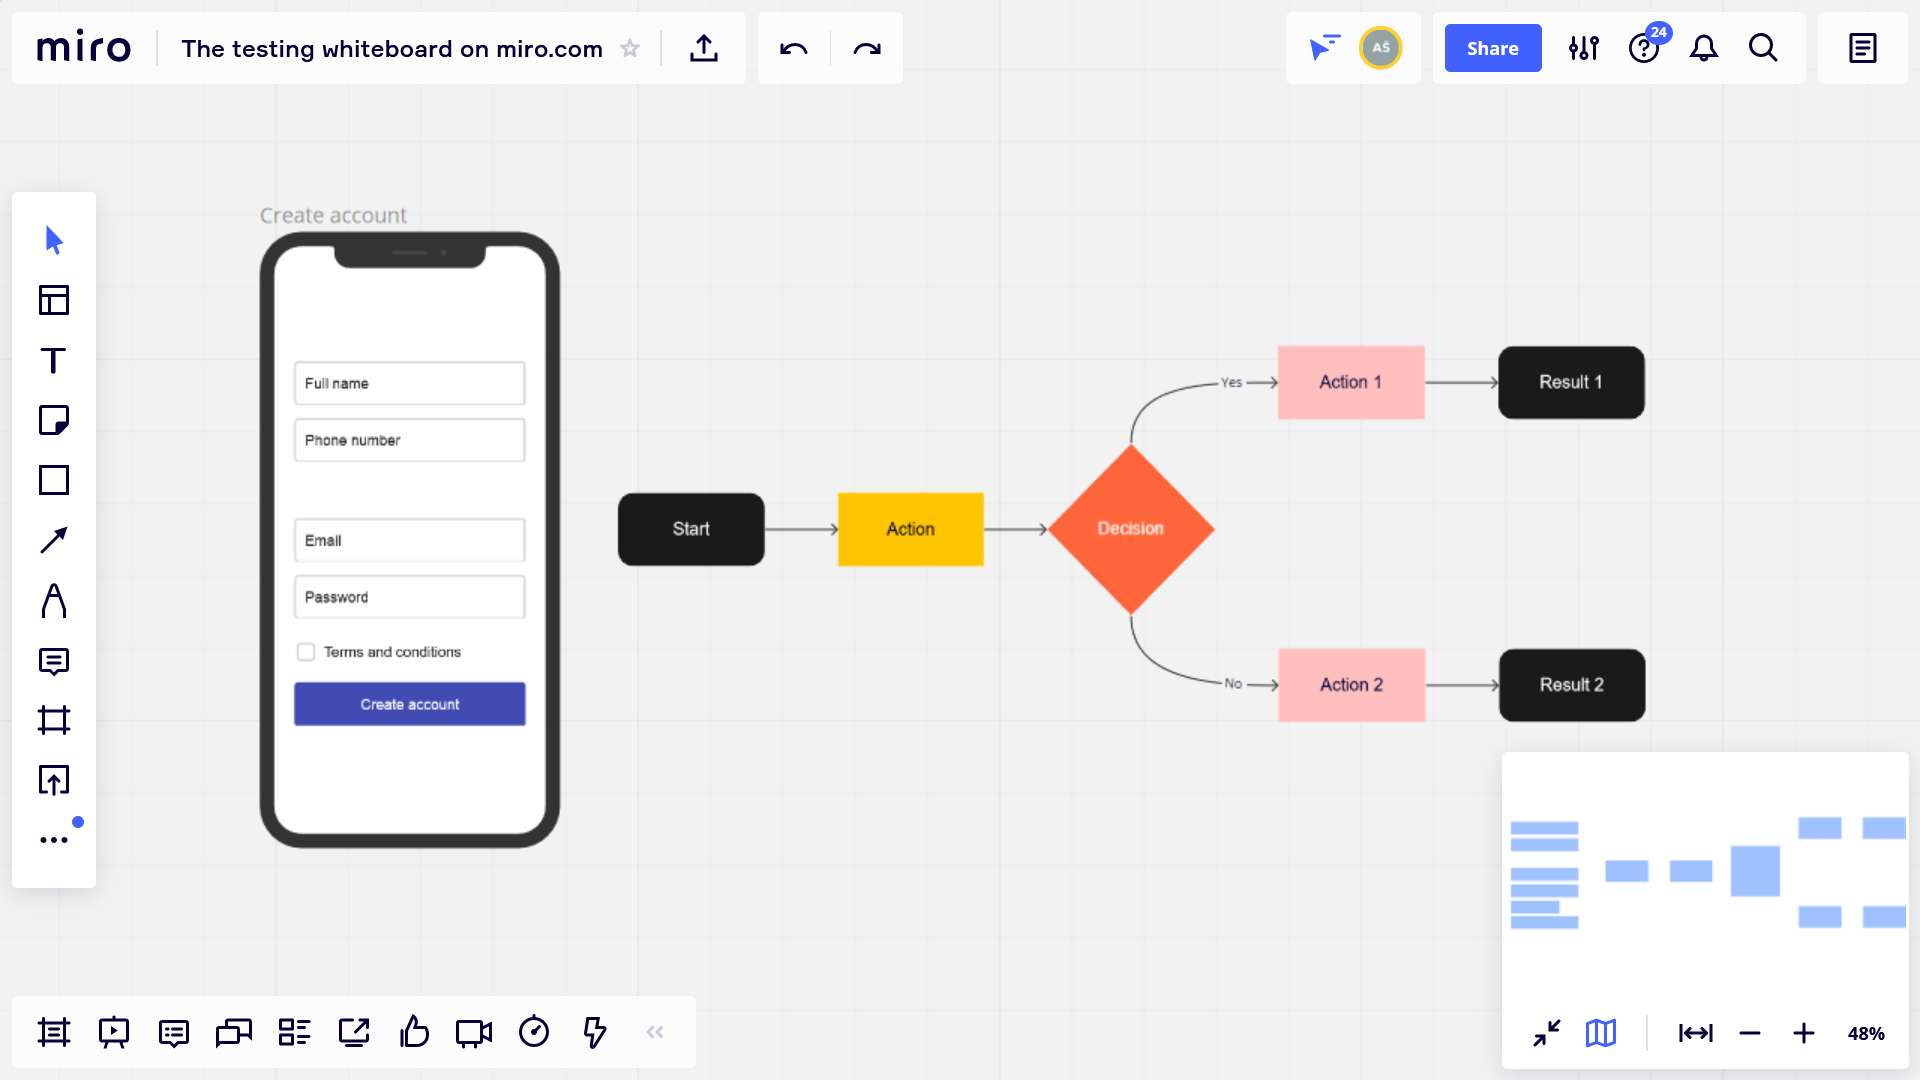
\includegraphics[width=1\textwidth]{Figures/miro.png}
	\caption{Ukázka webu miro.com}
	\label{fig:miro}
\end{sidewaysfigure}
\endinput
\chapter{Požadavky, analýza a návrh}
\label{chap:3}
\section{Požadavky}
\label{sec:3.1}
\subsection{Funkční požadavky}
\subsubsection{Diagram případů užití}
\begin{figure}[h!]
	\centering
	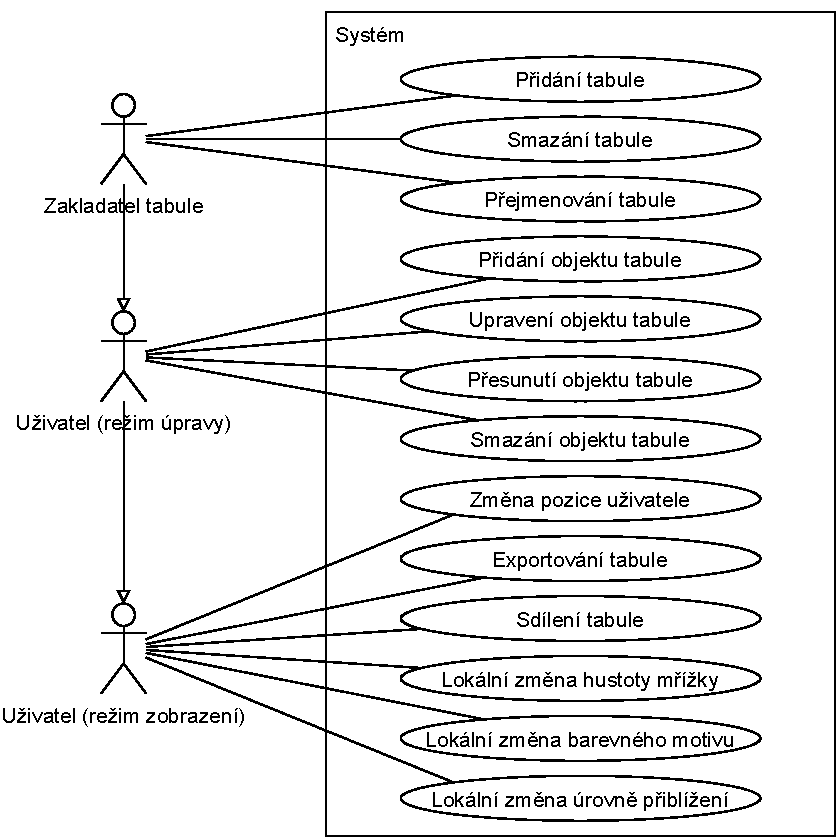
\includegraphics[width=0.6\textwidth]{Figures/UseCaseDiagram.pdf}
	\caption{Diagram případů užití}
	\label{fig:UseCaseDiagram}
\end{figure}
%#TODO Use-case / aktivitní diagram:
% + přidání tabule
% - přidání objektu tabule (lze dobře přidat rozšíření, kde bude odebrání objektu před kontrolou ID)
% - export tabule (obrázek)
% Sekvenční diagram:
% - přihlášení / připojení na tabuli
% + přidání obrázku
% - přidání zdrojového souboru
\clearpage


%#TODO\subsubsection{Scénáře případů užití}
%...


%#TODO\subsubsection{Aktivitní diagramy}
%#TODO\subsubsubsection{Aktivitní diagram - přidání tabule}
\subsection{Aktivitní diagram - přidání tabule}
\begin{figure}[h!]
	\centering
	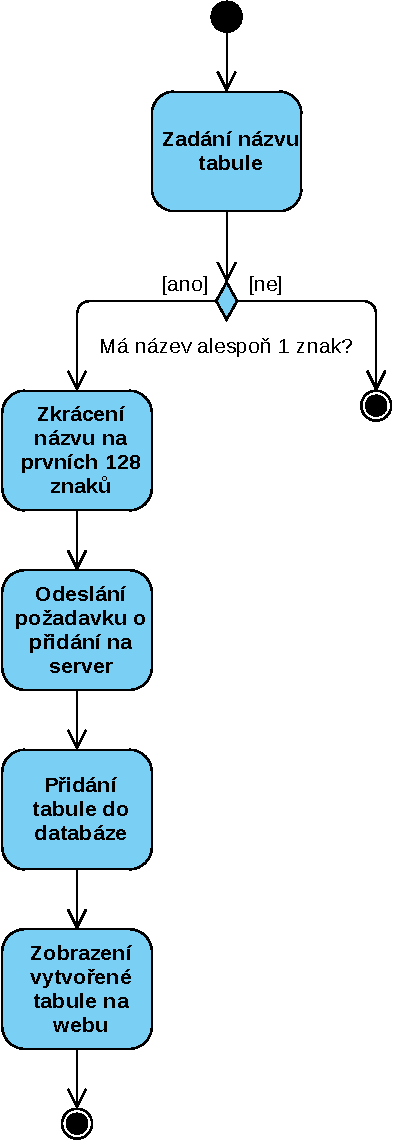
\includegraphics[width=0.33\textwidth]{Figures/ActivityDiagram1.pdf}
	\caption{Aktivitní diagram - přidání tabule}
	\label{fig:ActivityDiagram1}
\end{figure}
%#TODO...



%#TODO\subsection{Technické požadavky}
%\subsubsection{Konceptuální model domény (třídní diagram)}
%...


%#TODO\subsubsection{Odhad velikostí entit a jejich množství}
%#TODO...


%#TODO\subsubsection{Odhad počtu současně pracujících uživatelů}
%#TODO...


%#TODO\subsubsection{Typy interakcí uživatelů a odhad jejich náročnosti}
%#TODO...


%#TODO\subsubsection{Zvolené technologie a postupy}
%#TODO...
\clearpage




\section{Analýza}
\label{sec:3.2}
\subsection{Datová analýza}
\subsubsection{Relační datový model databáze}
\begin{figure}[h!]
	\centering
	%#TODO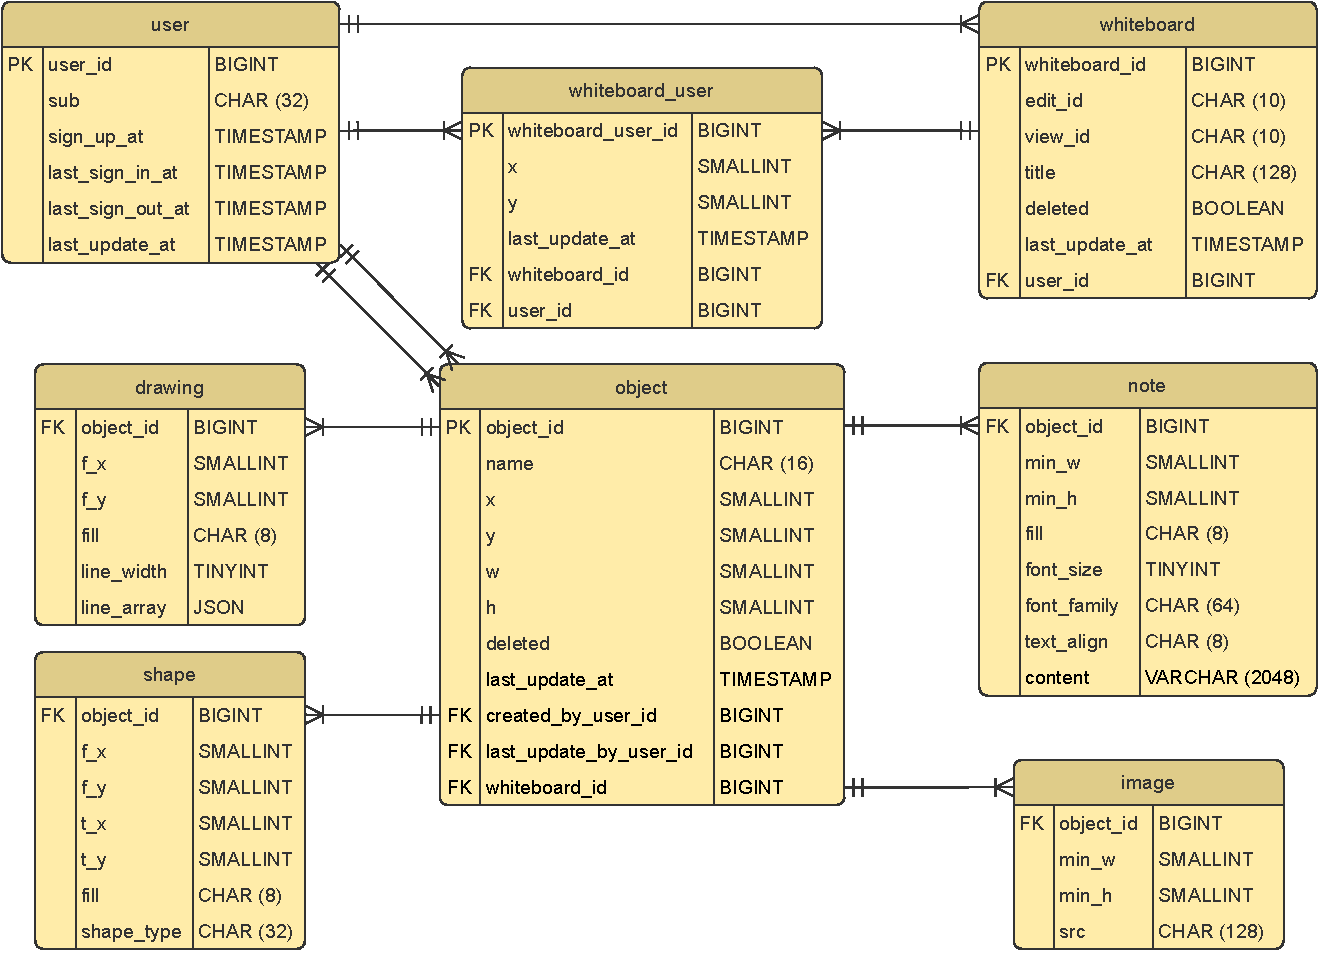
\includegraphics[width=1\textwidth]{Figures/EntityRelationshipDiagram.pdf}
	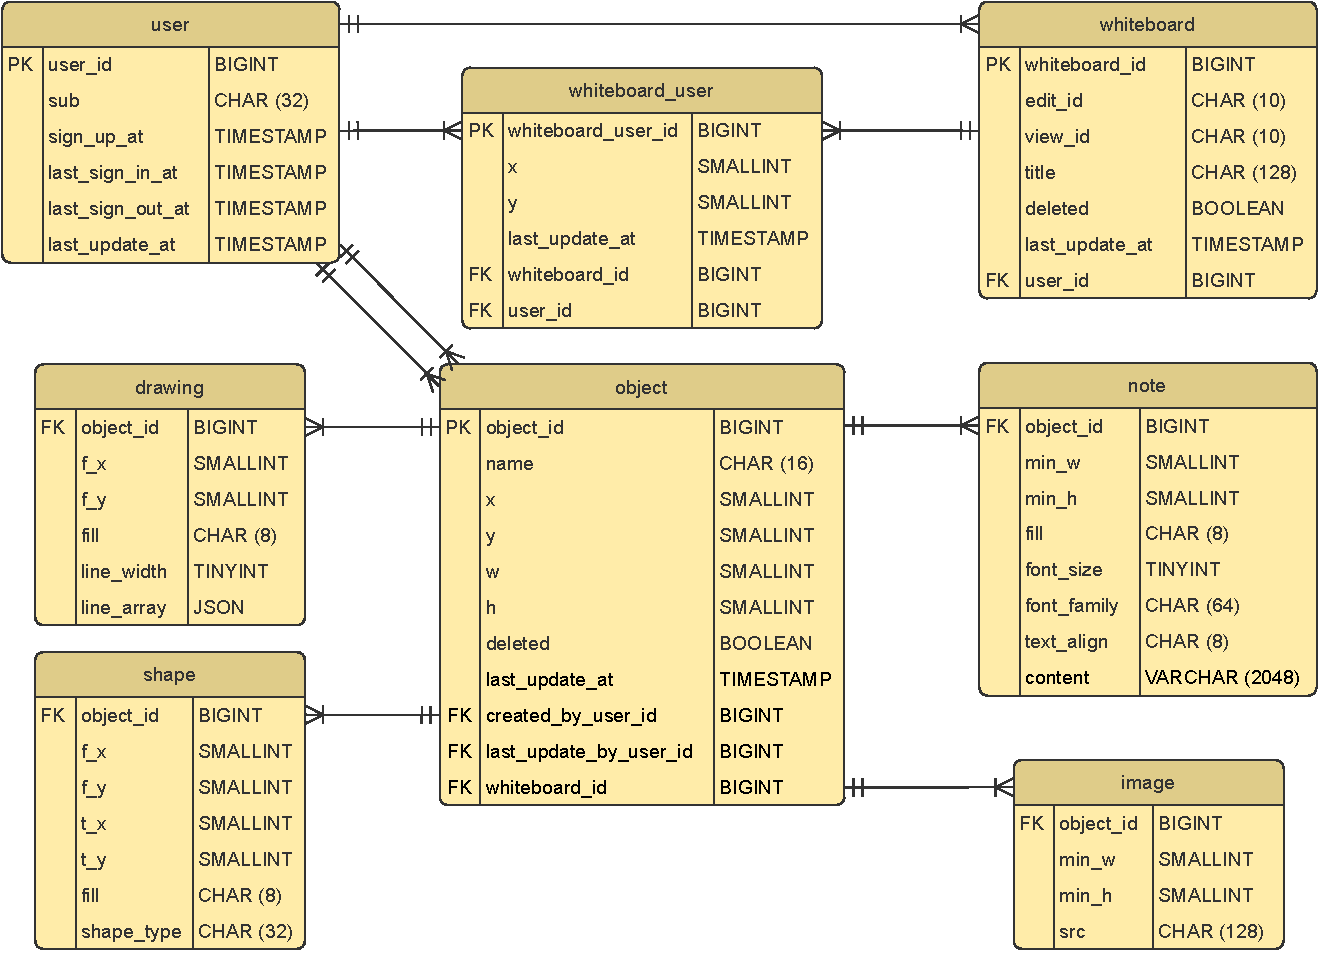
\includegraphics[width=0.9\textwidth]{Figures/EntityRelationshipDiagram.pdf}
	\caption{Relační datový model databáze}
	\label{fig:EntityRelationshipDiagram}
\end{figure}


%#TODO\subsubsection{Lineární zápis typů entit}
%#TODO...


%#TODO\subsubsection{Lineární zápis typů vztahů}
%#TODO...


%#TODO\subsubsection{Datový slovník}
%#TODO...


%#TODO\subsubsection{Integritní omezení}
%#TODO...



\subsection{Stavová analýza}
Definujeme tyto stavy tabule:
\begin{itemize}
	\item \textbf{Smazaná} -- tabule, která byla uživatelem smazána
	\item \textbf{Nesmazaná} -- tabule, která dosud nebyla uživatelem smazána
\end{itemize}

\noindent Definujeme tyto stavy objektu tabule:
\begin{itemize}
	\item \textbf{Smazaný} -- objekt tabule, který byl uživatelem smazán
	\item \textbf{Nesmazaný} -- objekt tabule, který dosud nebyl uživatelem smazán
\end{itemize}



%\subsection{Funkční analýza}
%...
\clearpage




\section{Návrh}
\label{sec:3.3}
\subsection{Architektura systému}
\subsubsection{Diagram nasazení}
\begin{figure}[h!]
	\centering
	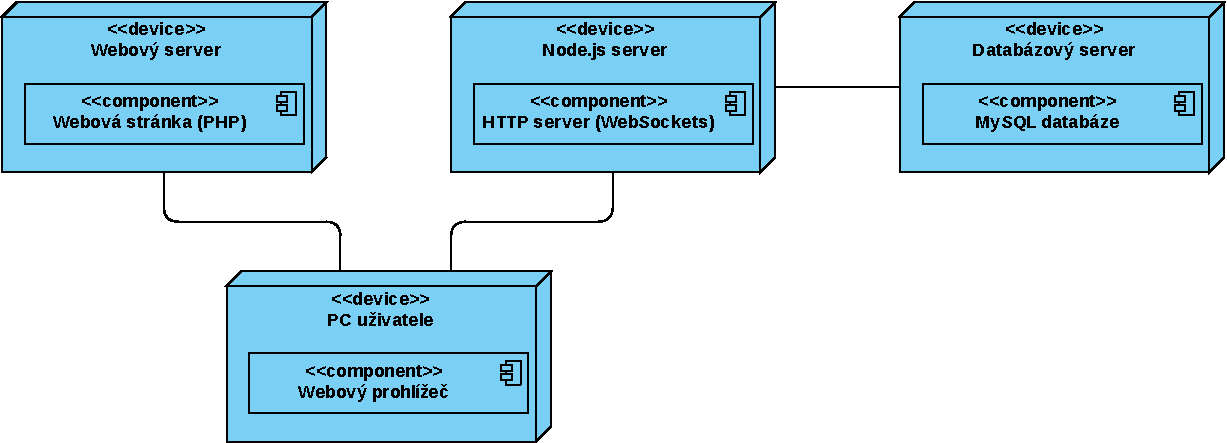
\includegraphics[width=1\textwidth]{Figures/DeploymentDiagram.pdf}
	\caption{Diagram nasazení systému}
	\label{fig:DeploymentDiagram}
\end{figure}


\subsubsection{Diagram komponent - datová komunikace}
\begin{figure}[h!]
	\centering
	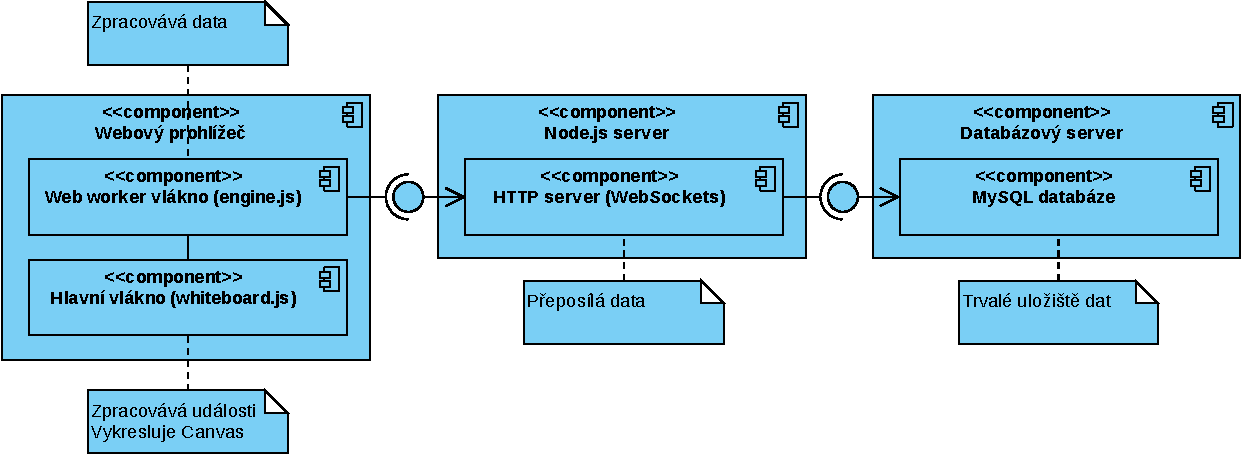
\includegraphics[width=1\textwidth]{Figures/ComponentDiagram.pdf}
	\caption{Diagram komponent - datová komunikace}
	\label{fig:ComponentDiagram}
\end{figure}
\clearpage



%#TODO\subsection{Sekvenční diagramy}
%#TODO\subsubsection{Sekvenční diagram - změna obrázku objektu tabule}
\subsection{Sekvenční diagram - změna obrázku objektu tabule}
\begin{figure}[h!]
	\centering
	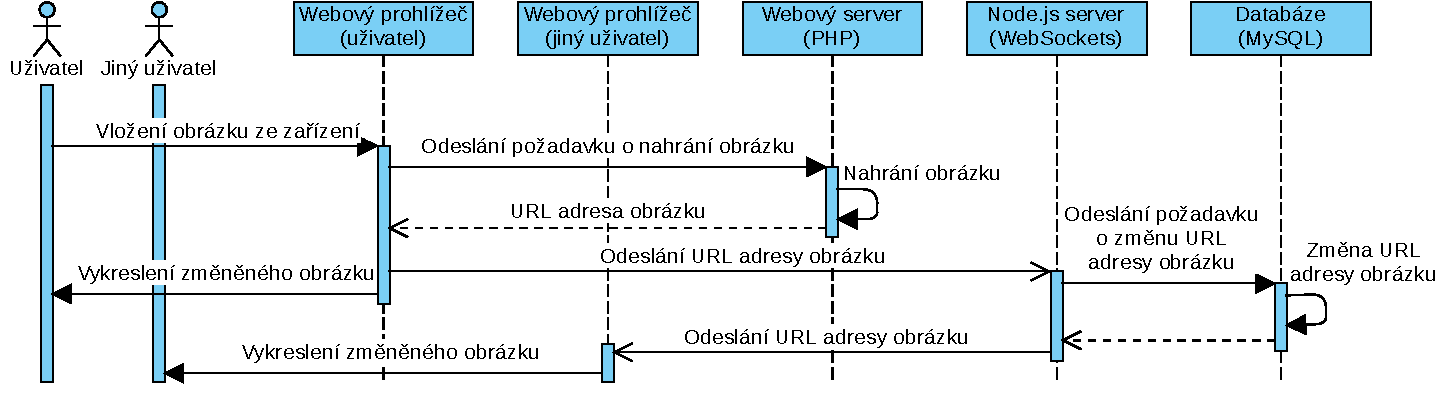
\includegraphics[width=1\textwidth]{Figures/SequenceDiagram1.pdf}
	\caption{Sekvenční diagram - změna obrázku objektu tabule}
	\label{fig:SequenceDiagram1}
\end{figure}
%#TODO...
\endinput
\chapter{Implementace}
\label{chap:4}
\section{Vykreslování grafického výstupu}
\label{sec:4.1}
\subsection{Zavedení Canvasu}
\begin{sloppypar*}
Pro vykreslování grafického výstupu je využíván HTML element \texttt{<canvas>}.
V JavaScriptu je objekt tohoto elementu možné získat pomocí DOM (objektový model dokumentu). \cite{web:MDN/DOM}
Získaný objekt \texttt{HTMLCanvasElement} je použit v rámci vlastní vytvořené třídy \texttt{WhiteboardCanvas}, která byla vytvořena za účelem optimálního vykreslování všech artefaktů tabule.
Nad objektem \texttt{HTMLCanvasElement} je zavolána funkce \texttt{getContext("2d")}, která vrací instanci rozhraní \texttt{CanvasRenderingContext2D}.
% CanvasRenderingContext2D => dvourozměrného vykreslovacího kontextu
Tato instance je pak dále nastavena všem již přidaným objektům tabule, které díky ní mohou začít vykreslovat.
\end{sloppypar*}

%\section{Využité zabudované funkce pro vykreslování}
%\begin{description}
%	\item[CanvasRenderingContext2D.clearRect()] -- funkce je využita k mazání obsahu tabule
%	\item[CanvasRenderingContext2D.fillText()] -- funkce je využita k vykreslování textu poznámky
%	\item[CanvasRenderingContext2D.fillStyle()] -- funkce je využita ke stylizaci výplně kreslených objektů tabule
%\end{description}



\subsection{Vykreslovací cyklus}
\begin{sloppypar*}
Vykreslovací cyklus probíhá v rámci již zmíněné třídy \texttt{WhiteboardCanvas}.
Cyklus začíná v metodě \texttt{linkHtml(canvas)} po získání instance \texttt{CanvasRenderingContext2D} zavoláním funkce \texttt{redraw()}.
\end{sloppypar*}
\begin{lstlisting}[language=JavaScript,label=src:JavaScript/WhiteboardCanvas.redraw(),caption={Metoda redraw() třídy WhiteboardCanvas}]
redraw() {
	if(this.redrawRequested) {
		this.clear();
		this.draw();
		this.redrawRequested = false;
	}

	requestAnimationFrame(this.redraw.bind(this));
}
\end{lstlisting}
\begin{sloppypar*}
Funkce začíná podmínkou, která kontroluje, zda je požadováno překreslení aktuálního stavu plátna.
Požadavek je při spuštění nastaven na hodnotu \texttt{true} právě z důvodu, aby počáteční vykreslení proběhlo bez nutnosti požadavek dále nastavovat.
\end{sloppypar*}
\begin{sloppypar*}
Pokud je podmínka splněna, dojde k vyčištění plátna a následnému vykreslení objektů přidaných funkcí \texttt{setObjects(objects)}.
Dále je pak požadavek nastaven na \texttt{false}, jelikož po aktuálním překreslení již další nejsou potřeba, dokud nedojde k nějaké změně, v rámci které bude tento požadavek vyvolán.
\end{sloppypar*}
\begin{sloppypar*}
Ať už podmínka byla nebo nebyla splněna, po jejím průchodu je, díky \texttt{requestAnimationFrame()}, funkce \texttt{redraw()} pokaždé znovu volána ve frekvenci odpovídající obnovovací frekvenci monitoru uživatele.
Díky omezení frekvence nemůže dojít k vyšším nárokům stránky (např. v módu kreslení), než které je koncové zařízení schopno zvládnout.
\end{sloppypar*}


\subsubsection{Odeslání požadavku o vykreslení}
\begin{sloppypar*}
Pokud dojde ke změně kterékoliv vlastnosti jakéhokoliv objektu tabule nebo se změní její barevný motiv je potřeba vyvolat požadavek o překreslení plátna skrze \texttt{requestRedraw()}.
\end{sloppypar*}
\begin{lstlisting}[language=JavaScript,label=src:JavaScript/WhiteboardCanvas.requestRedraw(),caption={Metoda requestRedraw() třídy WhiteboardCanvas}]
requestRedraw() {
	this.redrawRequested = true;
}
\end{lstlisting}
\begin{sloppypar*}
Nastavením proměnné \texttt{redrawRequested} na hodnotu \texttt{true} dochází v rámci vykreslovacího cyklu ke splnění podmínky, ve které následně dojde k překreslení plátna tabule.
\end{sloppypar*}



\subsection{Využití více vrstev pláten}
V rámci optimalizace byly místo jednoho Canvasu vytvořeny dva, jeden pro mřížku na pozadí a druhý pro samotný obsah tabule.
Důvod je jednoduchý. Plátno s mřížkou se aktualizuje méně často než hlavní vlákno.
Pokud by tedy byla mřížka s hlavním obsahem v jednom canvasu, musela by se pokaždé znovu překreslit i tato mřížka a zbytečně by tak byl snížen výkon webu.
%, což je redundantní proces, který by zbytečně snižoval výkon.
Plátno s vlastním obsahem tabule má průhledné pozadí, aby byla mřížka na pozadí viditelná.



\subsection{Využití vláken}
\begin{sloppypar*}
Součástí optimalizace řešení je využití současné práce více vláken.
JavaScript umožňuje kromě hlavního vlákna, které slouží především pro vykreslování a event handling, využít také další vlákna pomocí web workerů.
Tyto workery nemají přístup ke všem objektům, ke kterým má přístup hlavní vlákno, takže je nutné určité potřebné data poslat jiným způsobem.
To však není problém, jelikož workery mají přímo zabudovaný event \texttt{onmessage} pro příjem zpráv a funkci \texttt{send()} pro odesílání zpráv.
\end{sloppypar*}
Vedlejší vlákna jsou vhodná především pro větší výpočty či práci s daty, které nutně nemusí být v hlavním vláknu.
Čím méně instrukcí musí hlavní vlákno řešit, tím lépe zvládá činnosti, které je povinné zajišťovat.
Výsledkem je tedy plynulejší vykreslování a rychlejší reakce na jednotlivé události.

V této práci je využíváno pouze jedno vedlejší vlákno, jelikož je pro optimální funkčnost dostačující, nicméně je možné, že s pomocí více vedlejších vláken by šlo určité operace provádět současně a tedy efektivněji.


\subsubsection{Výpočet souřadnic}
Nejvíce výpočtů v práci souvisí s výpočtem souřadnic a je tedy vhodné tyto výpočty provádět v rámci vedlejšího vlákna.
Souřadnice jsou důležitou součástí zaznamenávání a zobrazování objektů tabule.
Práce k výpočtu souřadnic využívá několik faktorů, které ovlivňují, kde se zrovna uživatel nachází, jaká část tabule je viditelná a zda je vůbec samotný výpočet potřeba.

Výchozím referenčním bodem tabule je bod [0;0].
Tento bod označuje místo, kde se objevují noví uživatelé při prvním spuštění tabule a nachází se uprostřed uživatelovy obrazovky, ať už na počítači či mobilním zařízení.

Výhodou umístění bodu na střed je to, že je možné uprostřed vytvořit obsah, který má být pro nové uživatele na první pohled viditelný bez nutnosti se přepínat mezi záchytnými body tabule či se po tabuli přesunovat ručně.
Je to také místo, kde bude chtít začít většina uživatelů pracovat, takže bude výsledek viditelný ihned jednoduše pro všechny.

Dalším důvodem výběru je také to, že pokud by byl výchozí bod sice uprostřed tabule, ale tabule by souřadnice počítala pouze v kladných hodnotách, tak by objekty okolo středu měly zbytečně celkově vyšší hodnoty souřadnic.
Může se to zdát jako zbytečnost, nicméně při vyšším počtu tabulí, uživatelů a jejich dat toto může být důležitým opatřením pro udržení nižší datové náročnosti jak pro provozující server, tak pro internetové připojení klienta.
K tomuto přispívá nejen bod [0;0], ale také fakt, že veškeré souřadnice tabule jsou zaznamenávány v celých číslech.

Dalším rozhodnutím pro nižší datový přenos je omezení maximální velikosti tabule.
%Pro zajištění nižší náročnosti nejen pro přenos dat, ale také pro relativně rychlý export tabule je omezení maximální velikosti tabule.
Stávající maximální velikost tabule byla stanovena na rozlišení 32K z toho důvodu, že se dnes ještě nejedná o běžně dosažitelné rozlišení a tedy není snadné jednoduše vyčerpat celý prostor tabule.
Zároveň se však jedná o stále relativně nízké rozlišení pro exportování tabule do obrázku.
%Výhodou výběru tohoto bodu právě na střed je to, že je možné libovolně rozšiřovat obsah tabule do všech okolních směrů.
%Vybrat výchozí bod na střed je výhodné, jelikož se jedná o místo, kde lze vytvářet obsah viditelný pro nové uživatele a je možné se na tento bod kdykoliv přesunout pomocí tlačítka výběru důležitých míst tabule.
%, který je zároveň také místem, kde se objevují noví uživatelé, je bod [0;0].

\subsubsubsection{Faktor pozice uživatele}
Aby bylo možné vykreslit mřížku či libovolný objekt tabule, je nutné znát aktuální pozici uživatele.
Při prvním spuštění je tato pozice v bodě [0;0] nicméně díky možnosti se po tabuli pohybovat se tato hodnota v průběhu používání mění.
Pozice uživatele je vždy dána souřadnicemi bodu tabule uprostřed vykreslovaného plátna.
Při každé změně pozice je nutné souřadnice všech objektů přepočítat a znovu vykreslit aktualizovaný obsah.

\subsubsubsection{Faktor přiblížení}
Nejen pozice uživatele, ale i všech artefaktů tabule je ovlivněna také mírou přiblížení.
Přiblížit je možné až na úroveň 300~\% a oddálit pak na 30~\% standardní míry zobrazení.
S každým přiblížením či oddálením je rovněž nutné znovu přepočítat a vykreslit změny.

\subsubsubsection{Faktor velikosti obrazovky}
Velikost Canvasu ovlivňuje souřadnice událostí pracujících s pozicí kurzoru či prstu na obrazovce.
Vždy je nutné od aktuální pozice ukazatele odečíst polovinu velikosti Canvasu, čímž dojde k vycentrování ukazatele na střed a k dalšímu využití momentálních souřadnic uživatele.

Canvas také svojí velikostí udává viditelnou oblast tabule, kterou je nutné vykreslit, čímž je možné spoustu objektů tabule vynechat a nutné výpočty provádět pouze u zobrazených objektů.
Aby byl objekt považován za viditelný, je nutné aby byl alespoň jeden roh objektu ve viditelné oblasti.
Možným vylepšením současného stavu projektu je doplnění této podmínky o kontrolu skutečné vykreslené oblasti objektu.
Aktuálně se totiž může stát, že pokud např. objekt volného kreslení v daném rohu neobsahuje žádnou čáru, nicméně tento roh je součástí viditelné oblasti, tak se s tímto objektem počítá jako s viditelným a je nutné u něj vypočítat souřadnice i když ve výsledku na tabuli není vidět.
%zda se objeví objekt


\subsubsection{OffscreenCanvas}
OffscreenCanvas je experimentální technologie, která nově přináší vykreslování Canvasu pomocí Web workeru.
Kontext plátna není přímo závislý na DOM, což umožňuje jeho použití k vykreslování mimo hlavní vlákno. \cite{web:MDN/OffscreenCanvas}
%Bez použití této technologie renderování zmrazí veškeré ostatní operace v main threadu, dokud neproběhne vykreslování.
Přenesením renderovacích příkazů na vedlejší vlákno se eliminuje sekání způsobené vyčkáváním hlavního vlákna na dokončení vykreslovacích operací, které při plném využití výkonu znemožňují další interakci s webem.

Tato technologie je s použitím 2D kontextu zatím mezi nejrozšířenějšími prohlížeči podporovaná pouze prohlížeči postavenými na projektu Chromium a dále prohlížečem Samsung Internet, které globálně používá okolo 70\% uživatelů. \cite{web:CanIUse/OffscreenCanvas}

Jelikož podpora nezahrnuje prohlížeč Mozilla Firefox a další široce zastoupené značky, tak bylo po dohodě s vedoucím práce rozhodnuto tuto technologii neimplementovat a pouze její existenci zmínit v rámci tohoto dokumentu.

Podpora technologie OffscreenCanvas je však již nyní mezi vývojáři velmi žádaná a bude důležitou součástí webů využívajících Canvas.



\subsection{Vlastní třídy pro vykreslování}
Standardní metody rozhraní CanvasRenderingContext2D jsou plně postačující pro vykreslení několika jednoduchých tvarů.
Avšak pro využití ve větším počtu je v rámci zachování efektivity příkazů a přehlednosti zdrojového kódu lepší tyto funkce sjednotit.
Ke sjednocení byly použity třídy, které JavaScript podporuje od verze standardu ECMAScript 6.
%Nejedná se o jediný způsob, avšak tento byl vybrán z toho důvodu, že tyto třídy podporují dědičnost. Díky dědičnosti lze k problémům přistupovat pomocí OOP, což lépe strukturalizuje a zjednodušuje výsledný kód.

Seznam níže uvádí třídy, které byly v bakalářské práci vytvořeny za účelem zjednodušení či zefektivnění vykreslování jednotlivých artefaktů tabule:
\begin{sloppypar*}
\begin{description}
	\item[WhiteboardCanvasPolyline] -- Třída slouží k vykreslování lomené čáry. Tento typ čáry je využit k vykreslení mřížky a také v rámci nástroje kreslení, kde jedna lomená čára vyobrazuje jeden souvislý tah.\\
	V metodě \texttt{draw()} třída shlukuje příkazy \texttt{CanvasRenderingContext2D.moveTo()} a \texttt{CanvasRenderingContext2D.lineTo()} v rámci cyklu, který prochází zadané pole počátečních a koncových souřadnic čar. Cyklus čáry přidává do jedné cesty uvedené voláním \texttt{CanvasRenderingContext2D.beginPath()}, což zajišťuje efektivnější vykreslování, než kdyby byla každá čára vykreslována samostatně. \cite{web:HTML5Rocks/CanvasImprovePerformance}
	\item[WhiteboardCanvasRoundedRectangle] -- Třída slouží k vykreslování zaobleného obdélníku, který je použit jako pozadí poznámky. Výběr zaobleného obdélníku místo hranatého je čistě stylizační rozhodnutí.\\
	Třída v metodě \texttt{draw()} obsahuje, po volání \texttt{CanvasRenderingContext2D.beginPath()}, sekvenci 4 příkazů \texttt{CanvasRenderingContext2D.arc()}, které tvoří kruhové oblouky využité na zaoblené hrany obdélníku. \cite{web:MDN/CanvasRenderingContext2D/arc} Oblouky jsou následně spojeny zavoláním funkce \texttt{CanvasRenderingContext2D.closePath()}. \cite{web:MDN/CanvasRenderingContext2D/closePath} Spojení oblouků pomocí příkazu \texttt{closePath()} je efektivnější oproti samostatnému vykreslování zbylých čar na každé straně obdélniku. Celá nově vzniklá oblast je, dle nastavení v \texttt{CanvasRenderingContext2D.fillStyle}, vyplněna metodou \texttt{CanvasRenderingContext2D.fill()}. \cite{web:MDN/CanvasRenderingContext2D/fill}
	\item[WhiteboardCanvasText] -- Třída slouží k vykreslování textu poznámky.\\
	Canvas neumožňuje vykreslovat text na více řádků, takže je zdrojový HTML kód zpracován a rozdělen na jednotlivé řádky. Zarovnání dále nabízí pouze od daného bodu, takže je nutné pro zarovnání doprava a na střed tento výchozí bod posunout doprava resp. na střed poznámky. Jednotlivé řádky textu jsou poté zobrazeny pomocí metody \texttt{CanvasRenderingContext2D.fillText()}.
	\item[WhiteboardCanvasNote] -- Třída slouží k vykreslování poznámky. Obsahuje objekty tříd \texttt{WhiteboardCanvasRoundedRectangle} a \texttt{WhiteboardCanvasText}, díky kterým je možné poznámku vykreslit a obsahuje metody, jako např. \texttt{setPosition(x, y)} nebo \texttt{setSize(w, h)}, které oběma objektům nastaví potřebné vlastnosti. Cílem bylo zapouzdřit jednotlivé části poznámky do jedné třídy, pro snadnější úpravu libovolných parametrů.
	\item[ImageWrapper] -- Třída slouží k indikaci stavu načtení obrázku a umožňuje nastavit vlastní události \texttt{onerror(fn)} a \texttt{onload(fn)}. Dále obsahuje metodu \texttt{isReady()}, která říká, zda je obrázek načten (platí i při chybě při načítání) a \texttt{canDraw()}, která vrací \texttt{true} pouze v případě, pokud byl obrázek načten v pořádku.
	\item[WhiteboardCanvasImage] -- Třída slouží k vykreslování obrázku. Využívá objekt třídy \texttt{ImageWrapper}, jehož metody \texttt{isReady()} a \texttt{canDraw()} určí aktuální stav obrázku, který je pak následně zobrazen pomocí \texttt{CanvasRenderingContext2D.drawImage()}. Obrázek může nabývat následujících stavů:
	\begin{itemize}
		\item \textbf{Obrázek se načítá} -- je zobrazeno tmavě šedé pozadí s neutrálním piktogramem obrázku
		\item \textbf{Obrázek se nepodařilo načíst} -- je zobrazeno tmavě červené pozadí s piktogramem rozbitého obrázku
		\item \textbf{Obrázek byl úspěšně načten} -- je zobrazen samotný obrázek
	\end{itemize}
	\item[WhiteboardCanvasShape] -- Třída slouží k vykreslování geometrického tvaru.
	\begin{table}[h!]
		\centering
		\caption[Výpis tvarů a jejich volaných funkcí CanvasRenderingContext2D]{Výpis tvarů a jejich volaných funkcí CanvasRenderingContext2D}
		\label{tab:WhiteboardCanvasShape/CanvasRenderingContext2D/Functions}
		\begin{tabular}{ll}
			\toprule
			Tvar & Volané funkce CanvasRenderingContext2D\\
			\midrule
			Obdélník & \begin{sloppypar*}\texttt{beginPath()}, \texttt{rect()}, \texttt{fill()}\end{sloppypar*}\\
			Elipsa & \begin{sloppypar*}\texttt{beginPath()}, \texttt{ellipse()}, \texttt{fill()}\end{sloppypar*}\\
			Pravoúhlý trojúhelník & \begin{sloppypar*}\texttt{beginPath()}, \texttt{moveTo()}, \texttt{lineTo()}, \texttt{closePath()}, \texttt{fill()}\end{sloppypar*}\\
			Rovnoramenný trojúhelník & \begin{sloppypar*}\texttt{beginPath()}, \texttt{moveTo()}, \texttt{lineTo()}, \texttt{closePath()}, \texttt{fill()}\end{sloppypar*}\\
			Kosočtverec & \begin{sloppypar*}\texttt{beginPath()}, \texttt{moveTo()}, \texttt{lineTo()}, \texttt{closePath()}, \texttt{fill()}\end{sloppypar*}\\
			\bottomrule
		\end{tabular}
	\end{table}\\
	Tvary mají společné vlastnosti jako pozici, rozměry, pozadí a liší se pouze samotným typem tvaru.
	Jejich vykreslovací funkce tedy mohou být jednoduše rozděleny na základě typu tvaru přímo v rámci jedné třídy.
	Tímto se eliminuje duplikování totožných metod při vytváření samostatných tříd pro každý tvar zvlášť.
\end{description}
\end{sloppypar*}



\subsection{Barevné motivy tabule}
Dnešním trendem moderních webů a aplikací je podpora tmavého motivu.
Zatímco světlý motiv je vhodné využít především za ostřejšího denního světla, tak tmavý se hodí spíše v šeru večerních či nočních hodin, kdy je pro oči šetrnější.

Právě s denní dobou počítá ve výchozím stavu také vypracované řešení, kdy vždy v 18:00 se dle uživatelova lokálního času přepne web do tmavého motivu a ráno během 6:00 se zase opět vrátí do světlého motivu.
Toto automatické přepínání jde samozřejmě kdykoli tlačítkem přepnout přímo na výběr konkrétního motivu či vrátit zpátky na automatickou volbu.


\subsubsection{Barevný kontrast}
Vzhledem k tomu, že tmavé objekty na tmavém motivu a stejně tak světlé objekty na světlém motivu jsou špatně viditelné, tak se nabízí několik variant, jak tento problém vyřešit.

Jedním ze způsobů je zvolení daného motivu při vytváření tabule s tím, že by byl daný motiv nastaven pro všechny uživatele tabule a bez možnosti jej dále přepínat.
Tento způsob však není příliš ideální, jelikož si tímto uživatel de facto vyřadí právě jednu z funkcí, které web nabízí.

Dále je poté možné implementovat pouze světlý (nebo případně pouze tmavý) motiv.
Tento přístup lze pozorovat u téměř všech webů, kterými se práce inspirovala.
V rámci řešení však byla snaha najít vhodnou variantu, jak by se dalo implementovat oba barevné motivy a zároveň zachovat určitý barevný kontrast samotných objektů.

Při implementaci řešení tedy došlo k rozhodnutí, že aby byl obsah plátna dobře viditelný ať už na tmavém či na světlém motivu, které bude možné libovolně přepínat, tak bude potřeba zavést určité barevné odstíny.

\subsubsubsection{Zpracování barevného kontrastu}
\begin{figure}[h!]
	\centering
	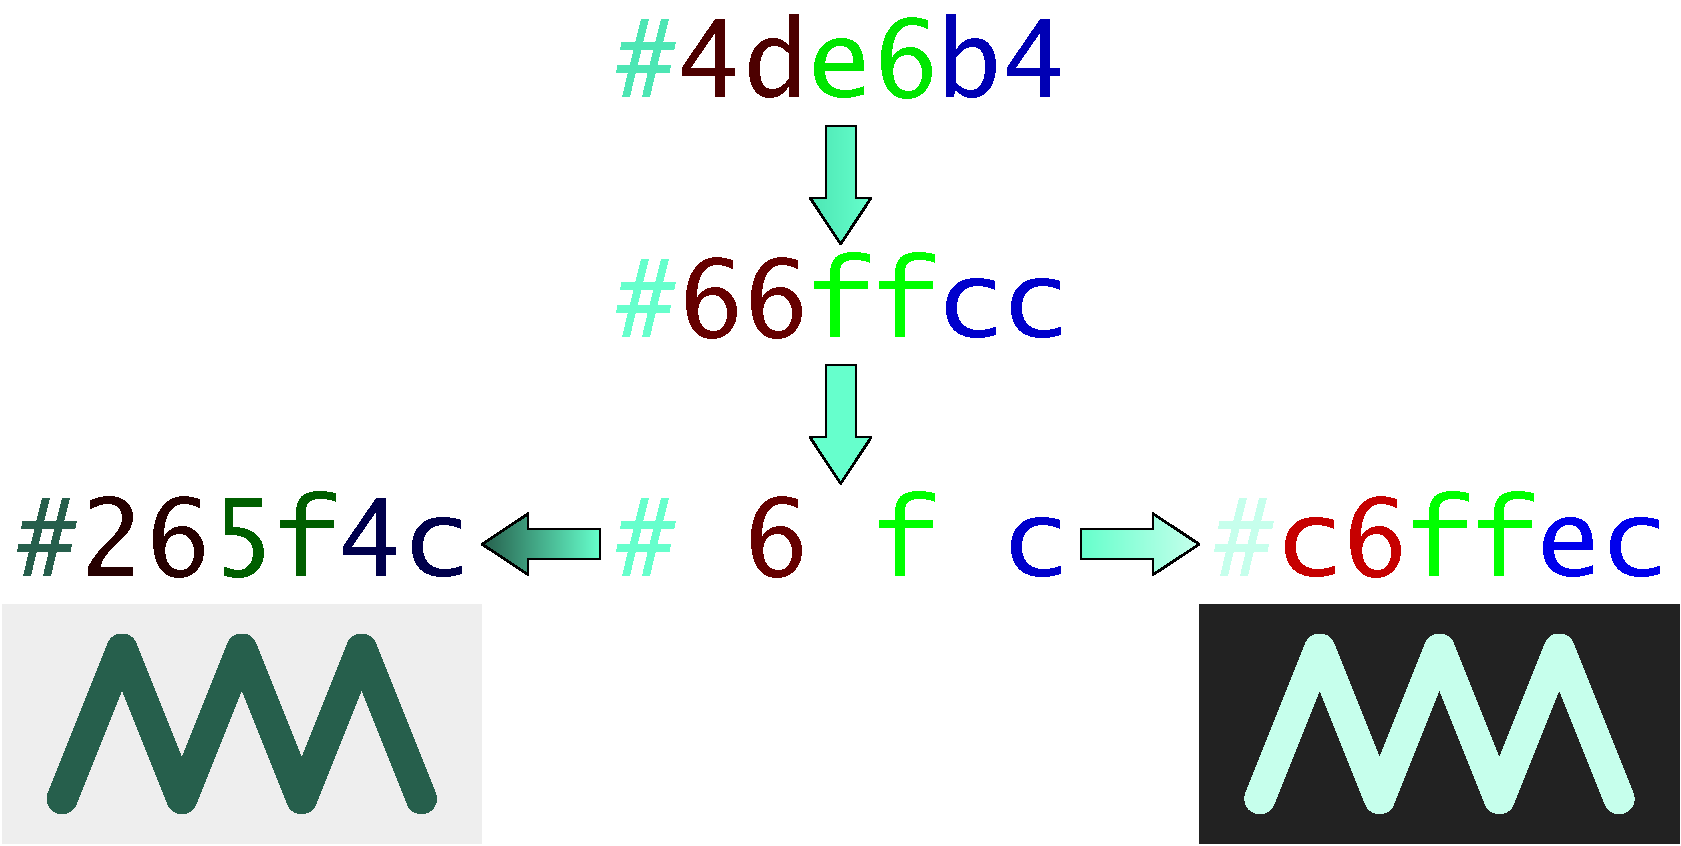
\includegraphics[width=0.5\textwidth]{Figures/colorMode.pdf}
	\caption{Příklad zpracování barvy \#4de6b4}
	\label{fig:colorMode}
\end{figure}

\begin{sloppypar*}
Jednotlivé objekty v rámci jejich vytváření či editace nabízí možnost změny barvy.
Pro výběr barvy je využit HTML element \texttt{<input type="color">}, který barvu vrací v hexadecimálním formátu \#rrggbb o barevné hloubce 24 bitů.
\end{sloppypar*}
Pro zesvětlení či ztlumení dané barvy je vrácený řetězec nejdříve převeden do 12 bitové barevného hloubky.
Tento krok je proveden převedením jednotlivých segmentů R, G a B do desítkové soustavy, vydělením 51, aritmetickým zaokrouhlením, vynásobením 3 a následně převedením zpět do hexadecimální soustavy.
%Jednotlivé části barev R (červená), G (zelená) a B (modrá) nabývají hodnot 00-FF, což po jejich převedení do desítkové soustavy znamená 0-255.
%Toto převedené číslo je následně vyděleno 51, aritmeticky zaokrouhleno, vynásobeno 3 a dále převedeno zpátky do hexadecimální soustavy.
Výsledkem těchto operací je hexadecimální řetězec, jehož 1.--2., 3.--4. a 5.--6. pozice obsahují stejný znak, a proto je možné jej zkrátit do formátu \#rgb.

Zkrácená varianta umožňuje vykreslit pouze 4~096 rozdílných barev, což je oproti původním 16~777~216 barvám veliký rozdíl.
Pokud by se jednalo o nástroj pro profesionální práci s grafikou, tak by tato barevná ztráta byla absolutně nepřípustná.
V tomto řešení však umožňuje právě již zmíněné zesvětlení či ztlumení barvy tím, že do zkrácené verze řetězce se opět, do každé ze 3 barev, přidá vždy zleva jeden znak.
Přidávané znaky zachovávají poměr jednotlivých barev od 0 do 5 a jsou případně zvýšené o požadovanou hodnotu od 0 do 10 tak, aby byly dostatečně viditelné v rámci daného motivu.
Obrázek \ref{fig:colorMode} graficky popisuje celý proces zpracování barev na uvedeném příkladu.

\subsubsubsection{Kontrast jednotlivých typů objektů}
Barevný odstín textu poznámky je stejný jako u vykreslovaných čar volného kreslení.
To stejné platí i o pozadí poznámky a pozadí geometrického tvaru.

Barevný odstín textu poznámky se pohybuje ve stejném rozmezí jako vykreslované lomené čáry u volného kreslení.
Důvodem stejného rozmezí je především charakter daných artefaktů, jelikož oba jsou velmi úzké a proto na tmavém pozadí by měly být světlejší a zároveň na světlém pozadí tmavší.

Pozadí poznámky i geometrického tvaru má rovněž stejné rozmezí, což je dáno tím, že zabírají relativně větší plochu a navíc u poznámky je nutné vzít v potaz také kontrast nejen vůči plátnu, ale také vůči samotnému textu poznámky.

%\subsubsection{Odstíny jednotlivých nástrojů}
%Tyto odstíny jsou součástí téměř všech typů objektů tabule kromě obrázku a při změně motivu se změny projeví přebarvením daného objektu do odpovídajícího odstínu dle barvy, kterou objekt obsahuje.



\subsection{Indikace upravovaných objektů}
Aktuálně upravované objekty tabule lze jednoduše rozeznat díky tomu, že jsou během úpravy barevně ohraničeny.
Barva ohraničení se liší na základě několika faktorů.
Pokud se jedná o objekt upravovaný aktuálním uživatelem v aktuálním okně, je ohraničení sytě růžové.
V případě, že jej sice upravuje aktuální uživatel avšak v jiném okně, je ohraničení zbarveno do šedě růžové barvy.
Šedé je pak ohraničení v případě, že daný objekt edituje úplně jiný uživatel.
Vykreslení barevného rámečku je čistě kosmetická záležitost, avšak samotný výběr objektu uživatelem je důležitá součást integrity tabule, která je dále podrobněji vysvětlena v následující kapitole.

\begin{figure}[h!]
	\centering
	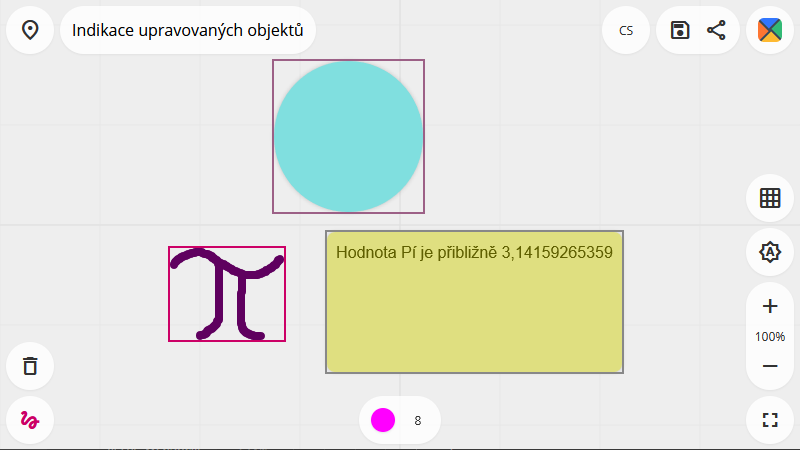
\includegraphics[width=1\textwidth]{Figures/ObjectIndication1.png}
	\caption{Pohled uživatele X v okně A (poloviční mřížka, světlý motiv, Mozilla Firefox)}
	\label{fig:ObjectIndication1}
\end{figure}

\begin{figure}[h!]
	\centering
	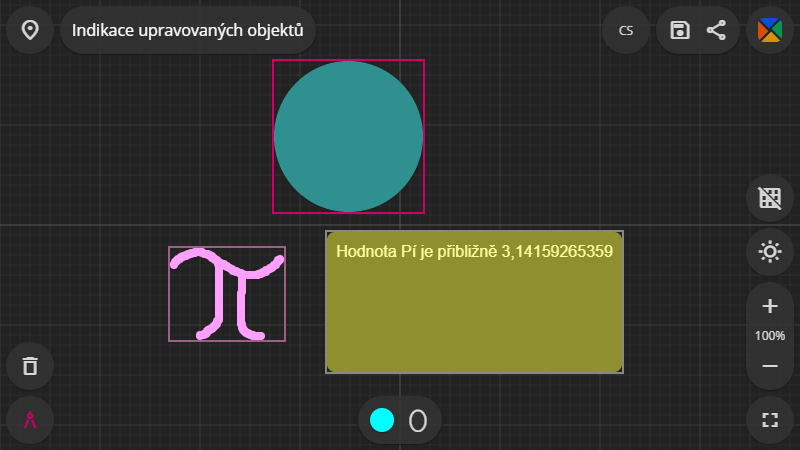
\includegraphics[width=1\textwidth]{Figures/ObjectIndication2.png}
	\caption{Pohled uživatele X v okně B (plná mřížka, tmavý motiv, Microsoft Edge)}
	\label{fig:ObjectIndication2}
\end{figure}

\begin{figure}[h!]
	\centering
	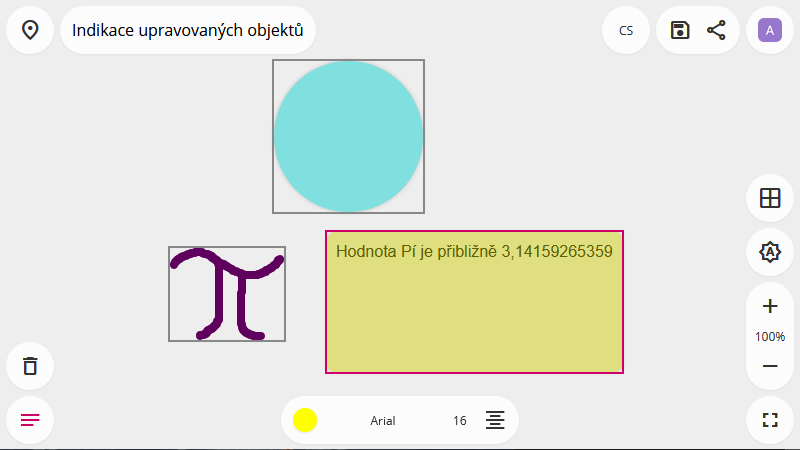
\includegraphics[width=1\textwidth]{Figures/ObjectIndication3.png}
	\caption{Pohled uživatele Y v okně C (žádná mřížka, světlý motiv, Mozilla Firefox)}
	\label{fig:ObjectIndication3}
\end{figure}
\clearpage




\section{Datová komunikace se serverem}
\label{sec:4.2}
Důležitou součástí webu je možnost spolupráce více uživatelů zároveň v reálném čase.
Sdílení dat je umožněno WebSocket serverem, který přijímá aktualizace jednotlivých detailů tabule a dále je rozesílá všem aktivně připojeným uživatelům kromě uživatele, který tuto změnu inicioval.
Součástí práce serveru je také ukládání dat do databáze či do proměnných o čemž pojednává následující sekce \ref{sec:4.3}.

%\section{Propojení jednotlivých částí webu}



\subsection{Součásti WebSocket serveru}
\subsubsection{Node.js}
Pro vývoj serverové části práce bylo vybráno prostředí Node.js.
Jedná se o asynchronní runtime JavaScriptu, který právě díky asynchronnímu přístupu umožňuje nenáročný vývoj škálovatelných síťových aplikací. \cite{web:NodeJS/About}
Node.js aplikace se programují v jazyce JavaScript a tyto aplikace je možné díky aktivní Node.js komunitě obohatit o již vytvořené balíčky, které celý vývoj zjednodušují.
Práce využívá ke svému fungování 4 balíčky uvedené níže:
\begin{itemize}
	%\item \textbf{express} -- slouží ke spuštění HTTP serveru na určitém síťovém portu, na který se poté klient připojuje
	\item \textbf{google-auth-library} -- určen k ověření klientského identifikačního čísla získaného po přihlášení k uživatelskému účtu Googlu
	\item \textbf{http} -- slouží ke spuštění HTTP serveru na určitém síťovém portu, na který se poté klient připojuje
	\item \textbf{mysql} -- umožňuje navázat komunikaci s MySQL databází
	\item \textbf{ws} -- zajišťuje komunikaci s klientským zařízením pomocí protokolu WebSocket
\end{itemize}


\subsubsection{WebSocket}
Technologie WebSocket byla vybrána z důvodu dlouhodobého spolehlivého spojení skrze plně duplexní komunikační kanál. \cite{book:AndrewLombardi/WebSocket}
Protokol vychází ze standardu RFC 6455 z roku 2011 a jeho aktuální podpora se pohybuje okolo 97--98~\% všech uživatelů webových prohlížečů. \cite{web:IETF/rfc6455}\cite{web:CanIUse/WebSockets}
%WebSocket protokol poskytuje plně duplexní komunikační kanál skrze jedno HTTP spojení a jeho definice vychází ze standardu RFC 6455 z roku 2011. \cite{book:AndrewLombardi/WebSocket}
%WebSocket API umožňuje jednoduché využití WebSocket protokolu pro komunikaci uživatelova prohlížeče a serveru. \cite{web:MDN/WebSocketAPI}


\subsubsection{JSON}
\begin{sloppypar*}
WebSocket protokol umožňuje přenos binárních či textových dat (kódování UTF-8). \cite{web:IETF/rfc6455}
K výměně dat práce používá datového formátu JSON, který pro přenos převádí na text pomocí příkazu \texttt{JSON.stringify()}.
JSON byl zvolen z důvodu snazšího debugování a vyšší přehlednosti výsledného kódu.
\end{sloppypar*}
Nižší velikosti odesílaných a přijímaných dat by bylo možné dosáhnout využitím binárních dat, nicméně jejich využití je vhodné po ujasnění výsledné formy všech posílaných dat.
JSON umožňuje rychleji a jednodušeji provádět změny struktury posílaných dat.



\subsection{Připojení uživatele}
Po vytvoření a spuštění je server připraven navázat spojení a komunikaci s webovou stránkou, pokud tato stránka splní určité přístupové kritéria.


\subsubsection{Validace údajů}
\subsubsubsection{Lokální část}
\begin{sloppypar*}
Prvním krokem před samotným pokusem o spojení je validace přístupových dat.
Nejprve je provedena kontrola URL adresy, tedy konkrétně, zda je uživatel připojen přes zabezpečený HTTPS protokol a zda celé doménové jméno odpovídá očekávaní.
Dále je pak ověřen řetězec přístupového režimu, který v adrese nabývá hodnot \textit{user}, \textit{edit} či \textit{view} a v případě posledních dvou také desetimístný unikátní identifikátor tabule pro daný režim.
Identifikátor se skládá z velkých a malých písmen anglické abecedy, číslic od 0 do 9 a dále pomlčky a podtržítka a je ověřen pomocí regexu \texttt{/\textasciicircum[A-Za-z0-9\textbackslash-\textbackslash\_]\{10\}\$/}.
Jako poslední je také provedena kontrola, zda se uživatel přihlásil a zda po tomto přihlášení byl získán potřebný token k dalšímu ověření na serveru.
\end{sloppypar*}
Toto základní ověření dat zajišťuje ochranu serveru před nežádoucími pokusy o připojení, především v případě možné interní chyby aplikace.
Pokud byly všechny výše uvedené podmínky splněny, webová stránka zažádá o připojení na WebSocket server a do připojované URL adresy zahrne GET požadavky s uvedenými kontrolními daty.

\subsubsubsection{Serverová část}
Na WebSocket server se může připojit prakticky kdokoliv, kdo zná jeho adresu, která je na webu lehce dohledatelná ve vývojářských nástrojích.
Nikdy tedy není možné předpokládat, že se uživatel připojuje pouze z konkrétního webu a také, že posílá smysluplné data.
Je tedy vhodné všechny vstupy ověřovat a při detekci jakékoliv anomálie uživatele odpojit od serveru buď úplně či případně s možností se znovu automaticky připojit v případě nějaké chyby aplikace.
\begin{sloppypar*}
Na serveru je tedy nejprve potřeba zkontrolovat původ připojovaného klienta, tedy opět zda se připojuje skrze HTTPS, z očekávaného webu, s použitelným režimem přístupu a v případě identifikátoru také jeho formátová správnost.
Token vrácený po přihlášení uživatele je následně pomocí balíčku \texttt{google-auth-library} verifikován a pokud je tato akce úspěšná, tak je získán unikátní identifikátor uživatelského účtu Google tzv. \texttt{sub}.
Po verifikaci je \texttt{sub} uložen do databáze (pouze v případě nového uživatele).
Poslední kontrola se týká pouze přístupových režimů edit a view a zjišťuje, zda se unikátní identifikátor tabule nachází v databázi.
%, ze které je pomocí příkazu \texttt{SELECT user\_id FROM user WHERE sub = \textquotesingle\$\{sub\}\textquotesingle LIMIT 1} vráceno uživatelské ID
%Je tedy nutné mít k přijímaným datům určitou míru nedůvěry a ověřovat co možná nejvíce  a je tedy nezbytné
%Pokud některá z předešlých podmínek není splněna, tak web dále nepokračuje v pokusu o připojení na WebSocket server.
%Toto základní ověření dat zajišťuje vyšší bezpečnost tím, že server chrání před nežádoucími pokusy o připojení.
%Jedná se však spíše o ošetření možných problémů aplikace než o pokročilou obranu před hackery.
%Práci je možné rozšířit mimo jiné právě o implementaci vyšší úrovně zabezpečení nejen na lokální úrovni.
\end{sloppypar*}


\subsubsection{Režimy přístupu}
\subsubsubsection{Režim uživatelského profilu}
- Přidání/editace/smazání více tabulí

\subsubsubsection{Režim editace tabule}
- Editace parametrů tabule (pouze její autor)\\
- Výběr objektu - editace, pohyb, smazání

\subsubsubsection{Režim zobrazení tabule}
- Osekaná verze režimu editace



\subsection{Udržování spojení}
- Ping/Pong
%\section{Příklady odesílaných dat}



\subsection{Důvody a řešení odpojení uživatele}

\subsubsection{Odpojení na základě chybné komunikace}

\subsubsection{Odpojení spojené s problémovým připojením k serveru}
- Výpadek serveru\\
- Výpadek internetového připojení uživatele
\clearpage

% výchozí pozice ve středu tabule je výhodná, jelikož:
% - umožňuje v budoucnu navyšovat maximální velikost tabule, která se zvětší do všech směrů a zároveň objekty i uživatelé zůstanou na původním místě (nebude třeba přepočítávat ze starých menších tabulí)
% - je možné se dále pohybovat do všech směrů
% - lze využít pro 
% - objekty u středu mají souřadnice blížící se k 0;0 a jsou tedy nižší než kdyby bylo možné se pohybovat pouze jedním směrem, kde by někteří uživatelé museli daleko zajíždět od počátku, aby mohli kreslit (ušetření dat)
% objekty jsou následně přepočítány do souřadnic canvasu


%Hlavním cílem je především zaměření na optimalizaci a efektivitu příkazů pro nerušené využití při spolupráci více uživatelů.
%Data jsou průběžně ukládána a načítána z databáze a pro jejich komunikaci mezi zařízeními je využito protokolu WebSocket.

% Další nápady:
% - kopírování objektů
% - přesouvání objektů do popředí po označení
% - místa uživatelů + přímo vytvořené checkpointy
% - změna velikost objektu
% - označení více objektů v rámci vybrané oblasti
% - přidání možnosti registrace pomocí emailu místo googlu a úprava profilu
% - přidání více možností přihlášení - microsoft, facebook, apple, github
% - ukládání do jiných formátů než jenom do JSON - např. XML
% - sdílení kromě emailu také přes facebook, twitter, instagram a další
% - přidání dalších jazyků kromě češtiny a angličtiny
% - přidání ikony/obrázku tabule, který by byl v pozvánce, ikoně záložky a na dalších místech
% - přidání chatu
% - přidání poznámek
% - offscreenCanvas

% Dotazy:
% - datum u citace odkazu - datum změny na webu nebo datum kdy jsem použil?
% - mám dobře dané citace v textu?
% - můžu takhle mít obrázky?




\section{Správa dat}
\label{sec:4.3}
\subsection{Správa dat na serveru}
\subsubsection{MySQL databáze}
% Pozice uživatele na tabuli


\subsubsection{Dočasné proměnné serveru}



\subsection{Lokální správa dat}
\subsubsection{Export tabule v nativní podobě formátu JSON}


\subsubsection{Nahrání obrázku pomocí Fetch API a PHP}


\subsubsection{Uložení uživatelských nastavení}
\subsubsubsection{LocalStorage}

\subsubsubsection{PHP Session}
\clearpage




\section{Uživatelské prostředí}
\label{sec:4.4}
\subsection{Uživatelské rozhraní}
\subsubsection{Řešení responzivity}


\subsubsection{Barevné motivy GUI}


\subsubsection{Jazyky GUI}



\subsection{Jednotlivé stránky webu}
\subsubsection{Stránka uživatelského účtu}
- Umožňuje přidání více tabulí...\\
- U každé tabule má tlačítka s odkazy na režim editace a zobrazení a smazání...


\subsubsection{Stránka s tabulí}
- Tlačítko pro přesouvání na důležité místa\\
- Tlačítka pro export a sdílení\\
- Tlačítko pro přepnutí na uživatelskou stránku či odhlášení\\
- Ovládání přiblížení tabule - zoom in/out/reset, fullscreen\\
- Tlačítka uživatelských nastavení - mřížka, barevné motivy, jazyk\\
- Tlačítka nástrojů tabule - kreslení, poznámka, obrázek, geometr. tvar, nativní podoba\\
- Rozdíly uživatelského rozhraní režimu editace a zobrazení


\subsubsection{Chybová stránka}
- Zobrazuje chyby 403, 404 a další...



\subsection{Sdílení tabule}
- Velmi krátká kapitola pouze o sdílení tabule, které nesedí do jiných kapitol\\
- Možnost zkopírování odkazu (bez dalších kroků, nejedná se o adresní řádek, ale o výběr možnosti v <select>)


\subsubsection{Sdílení emailem}
- Sdílení předem vytvořené zprávy v nastaveném jazyku - automaticky pomocí serveru (PHP funkce mail())\\
- Sdílení předem vytvořené zprávy v nastaveném jazyku - ručně uživatelem (mailto:)
\endinput
\chapter{Závěr}

\endinput

% Prilohy
\appendix
\chapter{Projekt}
Jednotlivé sekce přílohy byly vytvořeny za účelem doplnění zbývajících bodů požadavků předmětu Elektronické publikace. Ostatní požadavky již byly splněny v rámci samotného textu práce.

% Doplnění - zvýrazňování textu
\section{Zvýrazňování textu}
\textsc{Text psaný kapitálkami}



% Doplnění - výčtová prostředí
\section{Výčtová prostředí}
\begin{enumerate}
    \item První
    \item Druhý
    \item Třetí
\end{enumerate}

\newcounter{ListCounter}
\begin{list}{Část \Roman{ListCounter}:}{\usecounter{ListCounter}}
    \item Úvod
    \item Vypracování
    \item Závěr
\end{list}



% Doplnění - komentáře
\section{Komentáře}
\begin{comment}
    {\LARGE Obrovský text, který ale není vidět}
    \textit{Stejně tento vložený soubor!}
    \chapter{Úvod}
\label{chap:1}
Motivací práce bylo vytvořit moderní responzivní webovou aplikaci pro sdílení virtuální tabule, která bude umožňovat spolupráci více uživatelů na různých typech zařízení.
Virtuální tabule slouží k zaznamenávání a sdílení návrhů a ilustrací pomocí jednoduchých nástrojů, díky kterým je možné ji využít v práci, škole či v osobním životě.
%je oblast využití tohoto řešení skutečně široká.
Samotný obsah tabule je průběžně synchronizován, takže jsou změny jednotlivých uživatelů vidět přímo bez nutnosti stránku aktualizovat.
Zároveň jsou také veškeré úpravy ukládány do databáze, která slouží jako trvalé uložiště dat a také záloha při případném výpadku serveru či spojení.
%Databáze je poté využita pro načítání obsahu při připojení uživatele a také jako záloha při případném výpadku serveru či spojení.

%Myšleno je také na případné problémy, které se mohou vyskytnout nejen na straně uživatele, ale také na straně serveru.
%Samotný obsah tabule je průběžně synchronizován a ukládán, takže při výpadku sítě či serveru je po obnovení spojení vždy načten poslední uložený stav.
%, tak aby při , každopádně toto řešení nabízí také export pomocí obrázku či zdrojového souboru, kdykoli možné 
První kapitola se věnuje výběru jednotlivých stávajících řešení nástrojů pro sdílení virtuální tabule.
Kapitola uvádí nástroje a technologie vybraných webů a porovnává je s vypracovaným řešením.

Druhá kapitola se zaměřuje na rozbor požadavků, analýzu problémů a možných řešení a také na architekturu systému.
Kapitola přibližuje vnitřní strukturu systému na kterém je celé řešení postaveno.

Třetí kapitola pak pojednává o implementaci samotného řešení a jeho jednotlivých součástí.
Nejprve je zmíněno vykreslování, jeho optimalizace pomocí vláken a také zpracování barev v rámci barevných motivů.
Dále se kapitola věnuje výměně dat mezi klientských zařízením a serverem pomocí WebSockets.
Následně je popsána správa dat, která na lokální či serverové úrovni zajišťuje využití dat pro konkrétní potřeby uživatele.
Zmíněno je mimo jiné využití MySQL databáze, LocalStorage a Fetch API a také jednotlivé možnosti exportování tabule do rastrové či nativní podoby.
V poslední řadě se kapitola věnuje uživatelskému rozhraní z pohledu responzivity, podpory více jazyků včetně jejich zakomponování do sdílení tabule a také jednotlivým stránkám a jejich podobě ve finálním řešení.
%, ať už lokální či serverová zahrnuje využití MySQL databáze, LocalStorage či Fetch API a je pak dále včetně exportu tabule detailně popsána.
%S daty se lokálně i na serveru dále pracuje a tento proces je pak dále popsán včetně využití MySQL databáze, LocalStorage či Fetch API.  jsou následně ukládána do MySQL databáze či LocalStorage, což je také podrobně popsáno.
%Serverová i lokální správa dat je pak dále popsána včetně využití MySQL databáze a LocalStorage.
%začátek vývoje řešení, kdy 
%pojednává o využití Canvas API, coby plnohodnotné technologie pro vykreslování grafického výstupu na webu.
%Kapitola obsahuje popis této technologie včetně ukázky několika příkladů základních funkcí.

%Třetí kapitola se zaměřuje na výměnu dat mezi klientským zařízením a serverem pomocí protokolu WebSocket.
%Tento protokol poskytuje snadný a spolehlivý přenos dat, což umožňuje interaktivní spolupráci více uživatelů.

%Čtvrtá kapitola se věnuje správě dat a popisuje dva základní způsoby jak lze data ukládat či načítat pro další využití.
%Popsáno je využití MySQL databáze, kde data zůstávají uloženy dlouhodobě mezi jednotlivými návštěvami webu a dále pak exportování a nahrání dat v nativní podobě ve formátu JSON.

%Pátá kapitola rozšiřuje předchozí kapitoly o pohled na optimalizaci jednotlivých příkazů a dat, což umožňuje plynulejší chod webové aplikace.
%Zmiňuje se mimo jiné o Web workers použitých k rozdělení instrukcí do více vláken či o různých změnách v datech pro konkrétní místa použití.

%Poslední kapitola se zaměřuje na nedokončené části bakalářské práce a jejich možné rozšíření či vylepšení.
\endinput
\end{comment}



% Doplnění - vkládání vzorců
\section{Vkládání vzorců}
\begin{equation}
    E = mc^2
\end{equation}



% Doplnění - sazba indexu
\section{Sazba indexu}
Tento text je napsán v jazyce \LaTeX\index{\LaTeX}, který slouží k sazbě\index{sazba} dokumentu formy bakalářské práce\index{bakalářská práce} a také projektu do předmětu Elektronická publikace\index{ELP}.



% Doplnění - vkládání grafů z GNUplot
\section{Vkládání grafů z GNUplot}
Graf matematické funkce $x^2$:

\begin{gnuplot}[terminal=pdf,terminaloptions=color]
    unset key
    set samples 1000
    set format '%g'
    set xlabel "x"
    set ylabel "y"
    set xrange [-10:10]
    set yrange [0:100]
    plot x**2
\end{gnuplot}



% Doplnění - kreslení pomocí balíčku graphicx
\section{Kreslení pomocí balíčku graphicx}
\begin{figure}[h]
    \begin{center}
        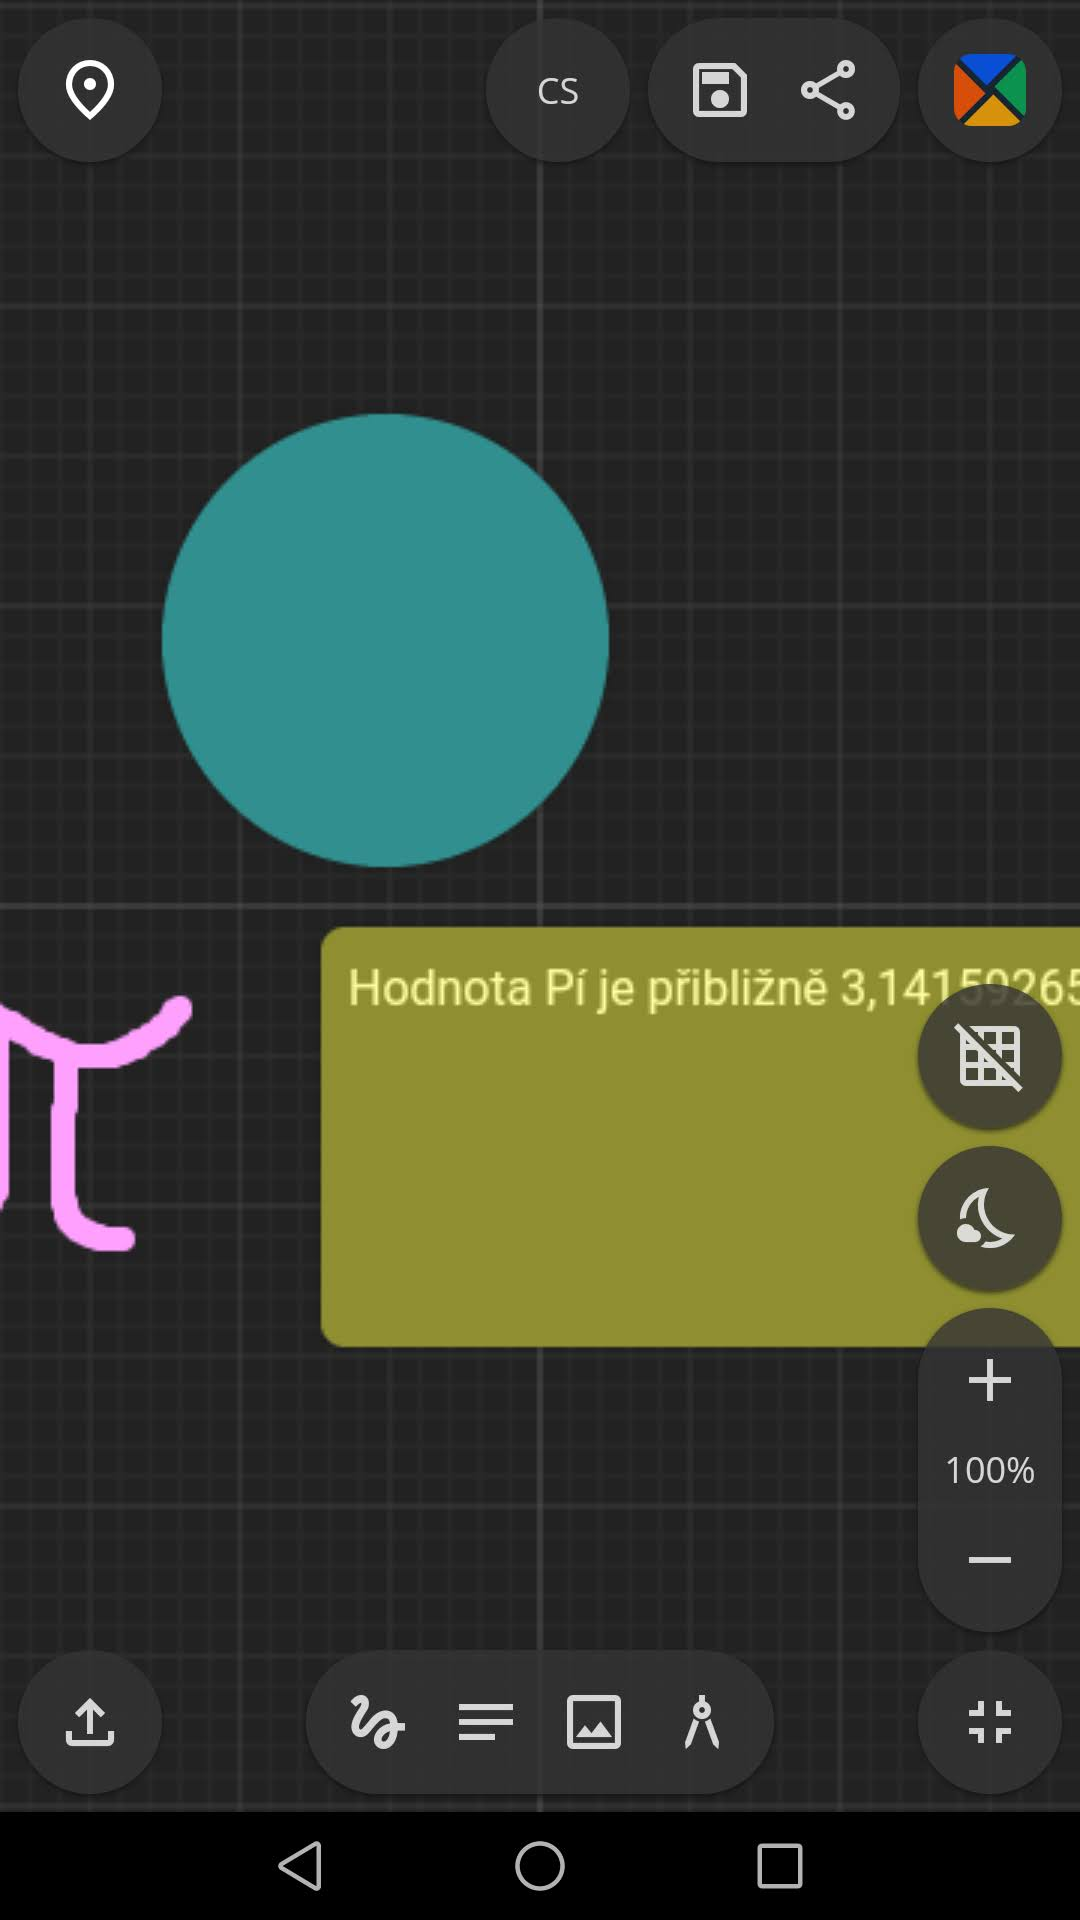
\includegraphics[height=0.5\textwidth, angle=80]{Figures/PhoneVersion.jpg}
        \caption{Obrázek otočený o 80\%}
        \label{fig:graphicx}
    \end{center}
\end{figure}



% Doplnění - sazba not
\section{Sazba not}
\begin{music}
    %\smallmusicsize
    \instrumentnumber{1}
    \setstaffs1{1}
    \generalmeter{\meterC}
    \nobarnumbers
    \startextract
    % bar 1
    \Notes \qu c \en                            % C
    \notes \ibu1d2\qb1d\tbu1\qb1e \en           % beamed DE
    \notes \ibu1g2\qb1f\qb1g%
        \qb1{'a}\tbu1\qb1b \en                  % beamed FGAB
    \bar % bar 2
    \Notes \ql{'c} \en                          % c
    \notes \ibu1{'b}{-3}%
        \qb1b\tbu1\qb1a \en                     % beamed BA
    \notes \ibu1{g}{-3}%
        \qb1g\qb1f\qb1e\tbu1\qb1d \en           % beamed GFED
    \bar % bar 3
    \notes \ibu1f0\qb1c\qb1g\qb1e\tbu1\qb1g%    % beamed CGEG
        \ibu1f0\qb1c\qb1g\qb1e\tbu1\qb1g \en    % beamed CGEG
    \bar % bar 4
    \Notes \qu c\qu e\qu c\qp \en               % CEC
    \endextract
\end{music}



% Doplnění - sazba exotických druhů písma
\section{Sazba exotických druhů písma}
\begin{itemize}
    %\item {\fontfamily{accanthis}\selectfont Písmo Accanthis}
    \item {\fontfamily{calligra}\selectfont Písmo Calligra}
    \item {\punkfamily\selectfont Písmo Punk}
    \item {\foekfamily\selectfont PISMO FOEKFONT}
\end{itemize}
\endinput

% Seznam literatury
\let\addspace\biblatexaddspace
\printbibliography[title={Literatura}, heading=bibintoc]

% Index
\printindex
\end{document}
